Tato kapitola se věnuje návrhu aplikace, tedy technologické architektury celé platformy a jednotlivých implementací, návrhu funkcionalit a uživatelskému rozhraní aplikace. V~následujících sekcích budou rozebírány jednotlivé navržené funkcionality a jejich rozhraní. Nejprve je ale potřeba si stanovit nějaký vzhledový styl aplikace.

Pro návrh uživatelského rozhraní aplikace byl použit nástroj \emph{Figma} \cite{figma}, dále byly použity zdroje z~šablony \emph{Apple Design Resources} \cite{apple-design-resources}. Zdroj všech návrhů lze nahlédnout v~\cite{trackee-app-figma}.

%---------------------------------------------------------------
\section{Vzhledový styl aplikace}
%---------------------------------------------------------------

Aplikace cílí na platformu iOS, což bude důležitou součástí jejího návrhu. Apple definuje rozsáhlou příručku pro návrh uživatelského rozhraní pro platformu iOS \cite{apple-design-guidelines-ios} a návrh aplikace se touto příručkou bude v~mnoha ohledech řídit.

Každá aplikace má nějaký svůj vzhledový styl, který definuje základní barvy, které bude aplikace používat, vzhledy tlačítek, textových polí, fontů a dalšího. Následující definice těchto prvků vychází převážně z~osobní preference, která se soustředí spíše na jednoduchost a ne příliš velkou výraznost rozhraní. Cílem tedy bude se přiblížit systémovému vzhledu platformy iOS a přidat vlastní mírný vzhledový jazyk.

%---------------------------------------------------------------
\subsection{Barvy}
%---------------------------------------------------------------

Základní návrh barev aplikace lze nahlédnout v~obrázku \ref{fig:colors}. Barvy jsou navrženy tak, aby vždy vznikl dostatečný kontrast mezi barvou pozadí a barvou popředí.

\begin{figure}[h]
	\centering
	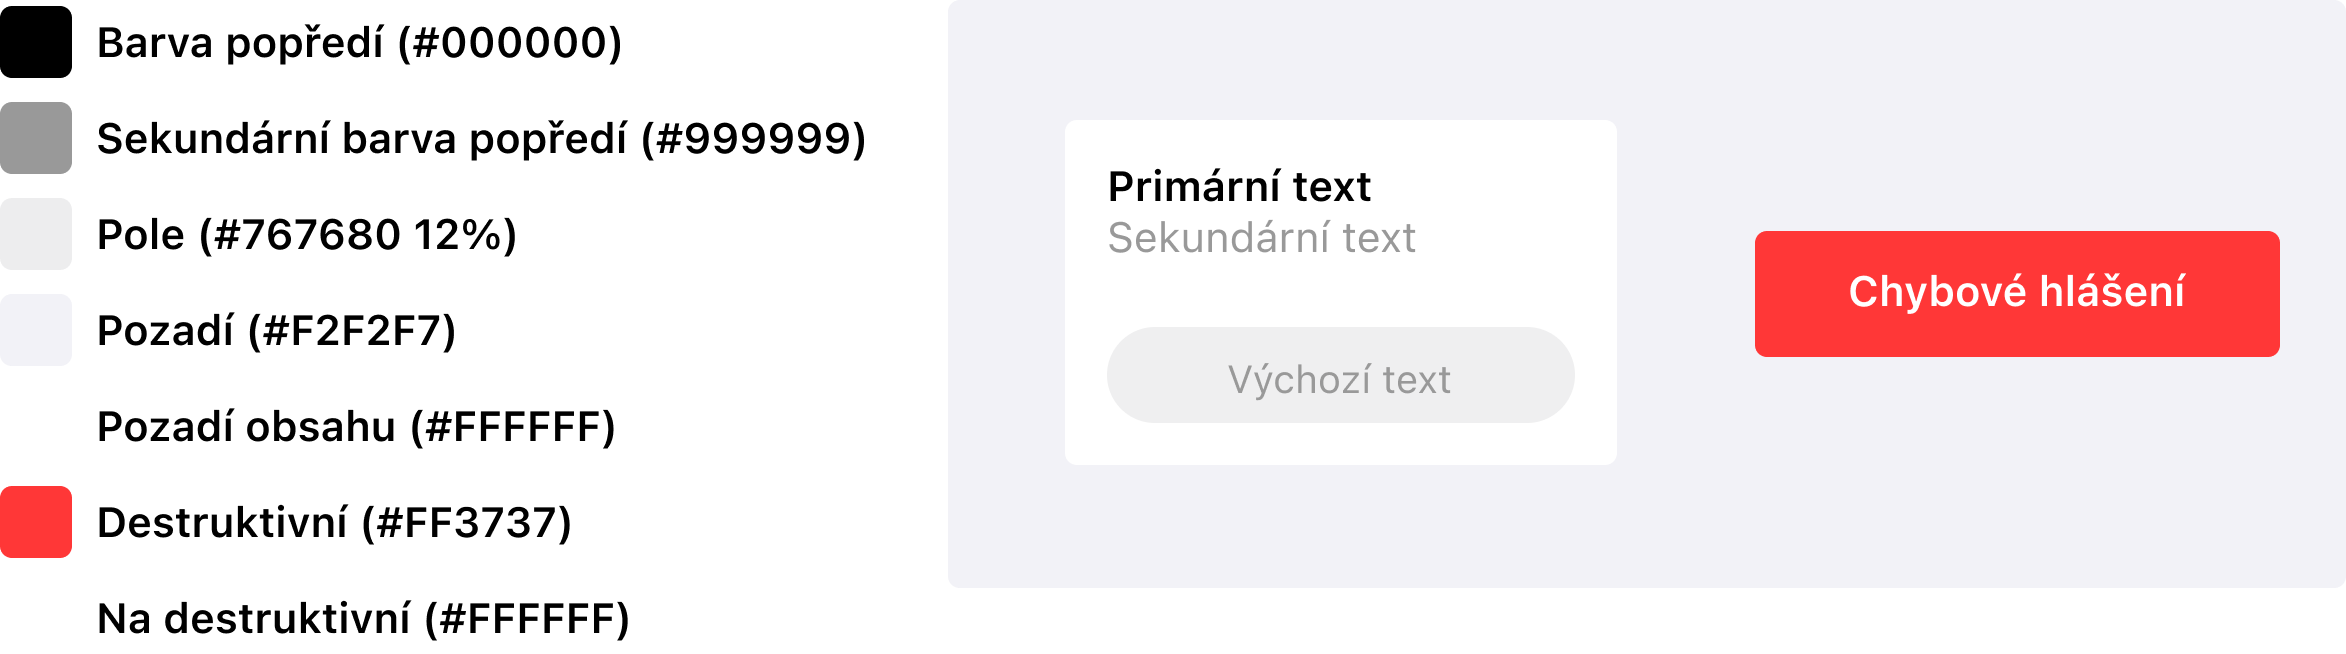
\includegraphics[width=\textwidth]{colors.png}
	\caption{Vzhledový styl aplikace – Barvy}
	\label{fig:colors}
\end{figure}

%---------------------------------------------------------------
\subsection{Fonty}
%---------------------------------------------------------------

Základní návrh fontů lze nahlédnout v~obrázku \ref{fig:fonts}. Daný font bude vždy používat systémovou rodinu fontů, tedy obvykle \emph{San Francisco} (SF). Jednotlivé velikosti jsou pouze referenční, protože aplikace by měla podporovat dynamické fonty a reflektovat tak škálování uživatele. Daná velikost je tedy velikost pro výchozí nastavení škálování textu.

\begin{figure}[h]
	\centering
	
\includegraphics[width=\textwidth]{fonts.png}
	\caption{Vzhledový styl aplikace – Fonty}
	\label{fig:fonts}
\end{figure}

%---------------------------------------------------------------
\subsection{Prvky}
%---------------------------------------------------------------

Návrh prvků rozhraní vychází z~již definovaných barev a fontů, lze jej nahlédnout v~obrázku \ref{fig:elements}.

\begin{figure}[h]
	\centering
	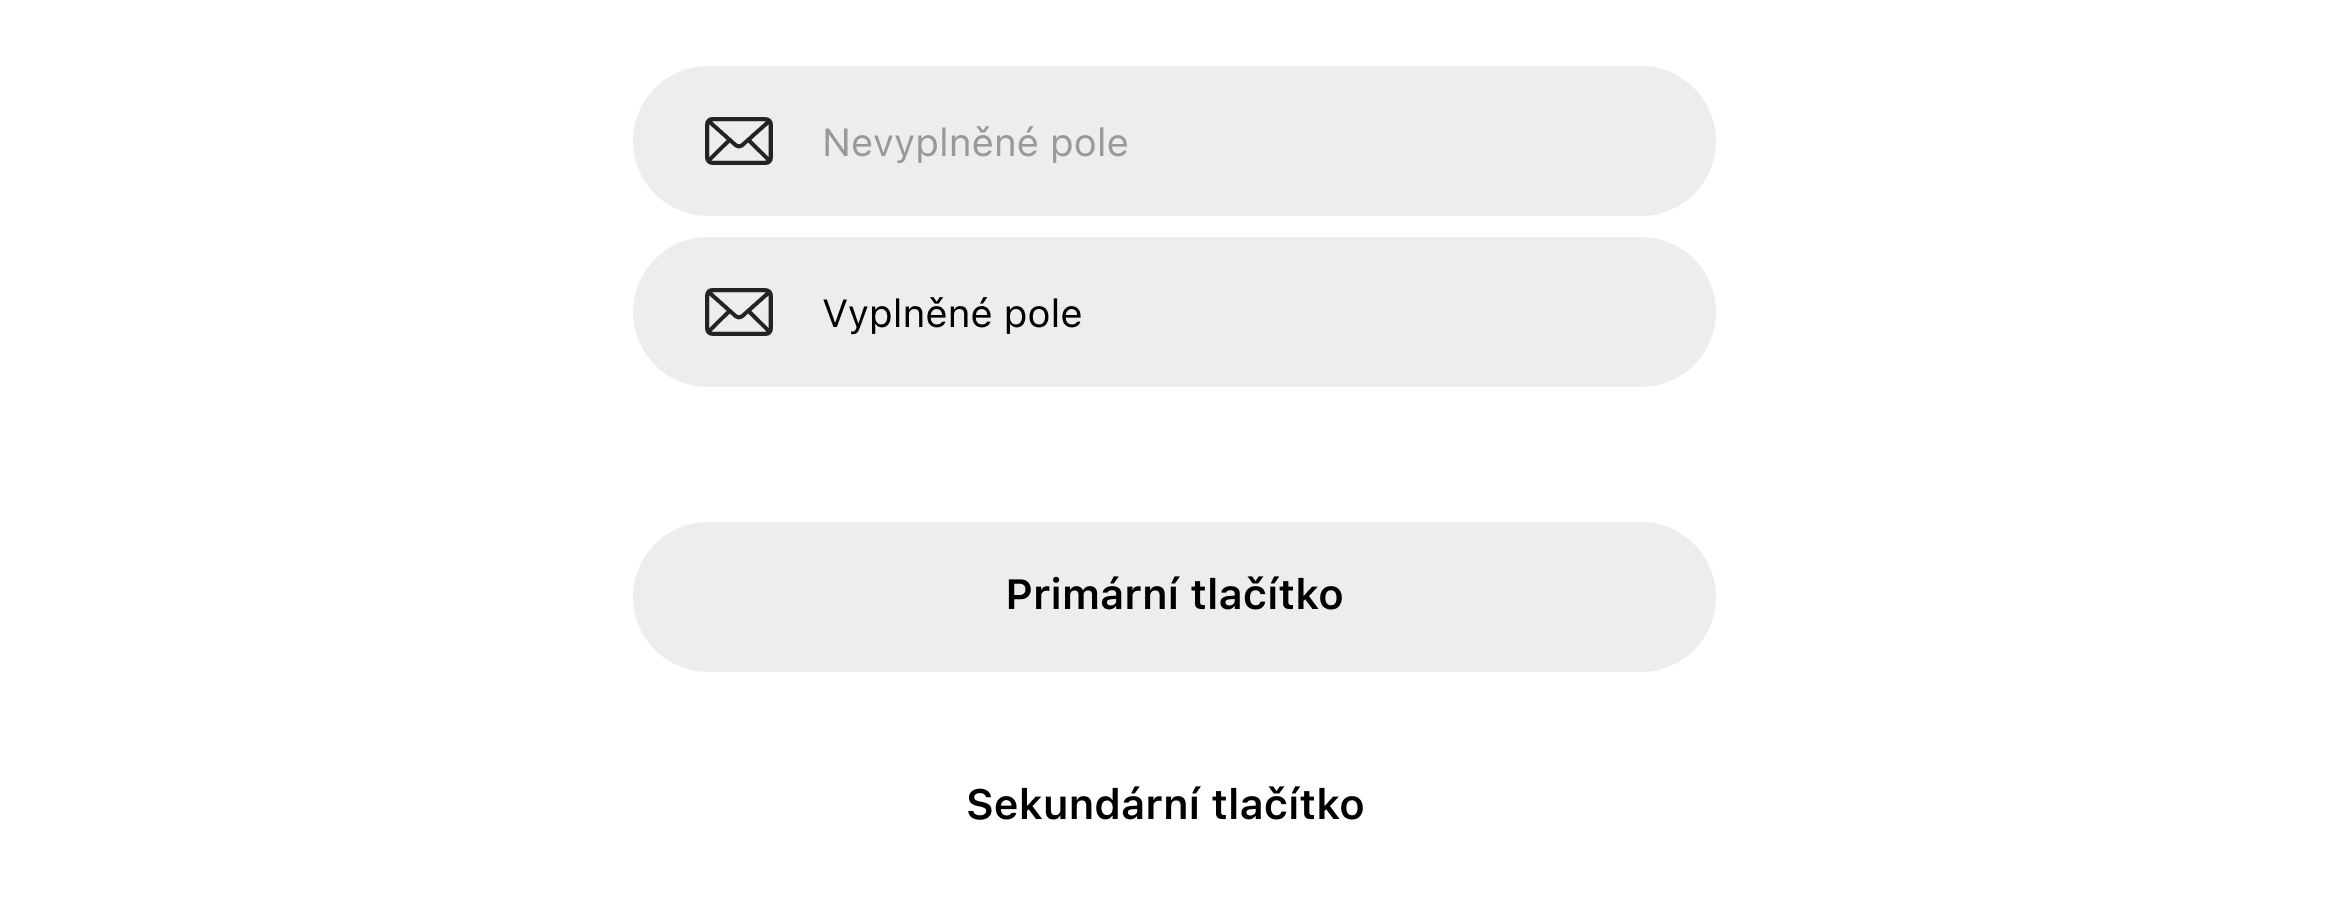
\includegraphics[width=\textwidth]{elements.png}
	\caption{Vzhledový styl aplikace – Prvky}
	\label{fig:elements}
\end{figure}

Na všechny ostatní prvky, jako prvky navigace, seznamy, alerty, a další, bude využito systémových prvků. Tím bude nejlépe vyhověno vzhledové příručce firmy Apple, pouze budou upravné některé barvy těchto prvků, aby ladily k~vzhledu aplikace.

%---------------------------------------------------------------
\subsection{Název a ikona}
%---------------------------------------------------------------

Návrh chytlavého názvu bývá obvykle složitá věc. Pro tuto aplikaci byl zvolen název \emph{Trackee} (anglicky [tra·ki]), který je odvozen z~anglického pojmu \emph{Time tracking}, což představuje měření odpracovaného času. Koncovka \emph{-ee} je také poslední dobou častou volbou pro názvy různorodých aplikací, jako \emph{Spendee} \cite{spendee}, \emph{Fondee} \cite{fondee} a další. Pod tímto názvem není registrována žádná ochranná známka \cite{upd-database}, ani není veden žádný záznam u~správce české domény \cite{cz-nic-trackee}.

Ikona aplikace také neprocházela nijak složitým procesem návrhu, byl pouze použit systémový symbol časovače na pozadí s~barvami aplikace popředí a pole. Ikonku lze nahlédnout v~obrázku \ref{fig:app-icon}.

\begin{figure}[h]
	\centering
	
\includegraphics[width=5cm]{trackee.png}
	\caption{Ikona aplikace}
	\label{fig:app-icon}
\end{figure}

%---------------------------------------------------------------
\section{Funkcionality aplikace a jejich uživatelské rozhraní}\label{features}
%---------------------------------------------------------------

Aplikace bude primárně sloužit pro zaznamenávání odpracovaného času. Je tedy potřeba, aby každý uživatel měl možnost si vytvářet vlastní záznamy a další data, která budou propojena pouze s~ním, a ke kterým bude mít přístup pouze on. Toto obvyklý případ užití mobilní aplikace, který ze své podstaty vyžaduje nějakou formu vytvoření uživatelského účtu, se kterým budou data propojena, a jeho autentizace. Nejobvyklejším způsobem autentizace je autentizace pomocí e-mailu a hesla. Tento způsob je i~poměrně jednoduchý z~hlediska implementace a spousta poskytovatelů BaaS (Backend as a Service, vizte \ref{baas}) tento způsob autentizace implementuje. 

%---------------------------------------------------------------
\subsection{Přihlášení a registrace}\label{feature-onboarding}
%---------------------------------------------------------------

Tato funkcionalita bude sloužit pro následující případy užití:
\begin{itemize}
\item\textbf{Přihlášení} – Uživatel se přihlásí pomocí e-mailu a hesla.
\item\textbf{Registrace} – Uživatel si vytvoří účet pomocí e-mailu a hesla.
\end{itemize}

Přihlašovací obrazovka bude obsahovat pouze nadpis, pole pro vyplnění e-mailu, hesla, primární tlačítko pro přihlášení a sekundární tlačítko pro registraci. Obrazovka pro registraci, která se otevře po kliku na tlačítko pro registraci, poté bude od uživatele potřebovat také jen e-mail a heslo, které je ale zvykem napsat dvakrát, aby se snížila šance, že se v~něm vyskytl překlep. Obrazovky přihlášení a registrace lze nahlédnout v~obrázku \ref{fig:onboarding}. Úspěšné přihlášení a registrace uživatele přesměruje na hlavní obrazovku aplikace.

\begin{figure}[h]
    \centering
    \begin{subfigure}[b]{0.4\textwidth}
		\centering
		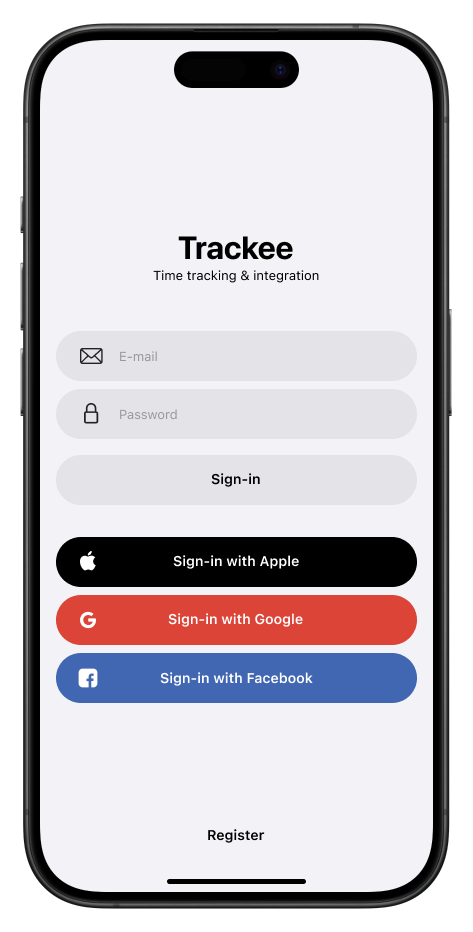
\includegraphics[width=6cm]{login.png}
		\caption{Přihlášení}
		\label{fig:login}
	\end{subfigure}
	\hspace{2cm}
	\begin{subfigure}[b]{0.4\textwidth}
		\centering
		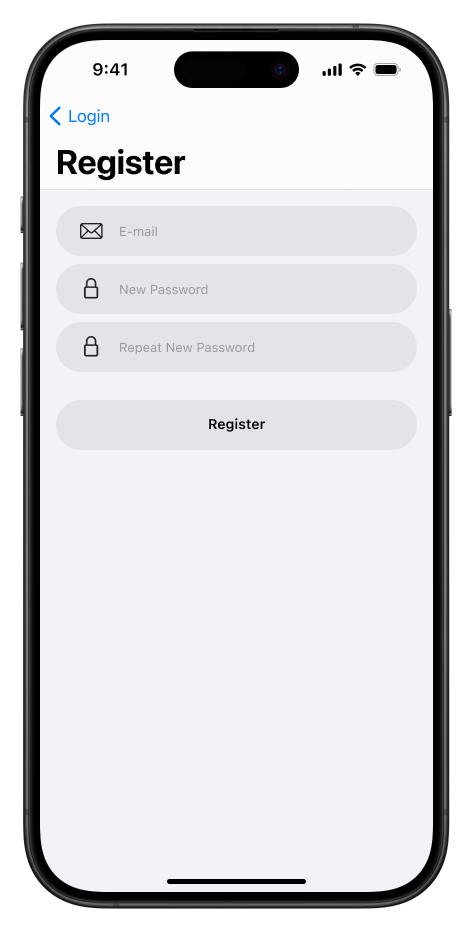
\includegraphics[width=6cm]{register.png}
		\caption{Registrace}
	\end{subfigure}
	\caption{Onboarding}
	\label{fig:onboarding}
\end{figure}

%---------------------------------------------------------------
\subsection{Lišta karet a časovač}\label{feature-timer}
%---------------------------------------------------------------

Funkcionalita časovače bude sloužit pro následující případy užití:
\begin{itemize}
\item\textbf{Zapnutí časovače} – Uživatel spustí časovač a začne tak měřit odpracovaný čas.
\item\textbf{Výběr projektu} – Uživatel přiřadí projekt k~záznamu, který chce měřit nebo vytvořit.
\item\textbf{Zadání popisu} – Uživatel zadá popis k~záznamu, který chce měřit nebo vytvořit.
\item\textbf{Zastavení časovače a uložení záznamu} – Uživatel zastaví časovač a uloží tím záznam, který do zastavení měřil.
\item\textbf{Manuální přidání záznamu} – Uživatel vytvoří nový záznam podle zadání času začátku a konce.
\item\textbf{Odstranění záznamu} – Uživatel odstraní časový záznam z~historie. 
\item\textbf{Zobrazení historie záznamů} – Uživatel si prohlédne libovolné záznamy z~historie.
\item\textbf{Zobrazení shrnutí odpracovaných hodin} – Uživatel si zobrazí souhrn odpracovaných hodin daného dne nebo současného týdne.
\end{itemize}

Navigace mezi hlavními obrazovkami aplikace bude řešena pomocí lišty karet, jelikož se jedná o~častý a doporučený způsob, jak navigovat mezi vzájemně exkluzivními částmi obsahu \cite{apple-guidelines-tabbars}. Hlavní obrazovkou bude přehled, na kterém bude uživatel moct ovládat časovač, a kde uvidí historii svých časových záznamů, seřazenou od nejnovějších po nejstarší. Jelikož pro uživatele je nejjednodušší dosáhnout na ovládací prvky, které jsou ve spodní části displeje, bude ovládání časovače umístěno ve spodní části obrazovky, a časové záznamy se budou řadit nad ním. Návrh této obrazovky lze nahlédnout na obrázku \ref{fig:timer}.

\begin{figure}[h]
    \centering
    \begin{subfigure}[b]{0.4\textwidth}
		\centering
		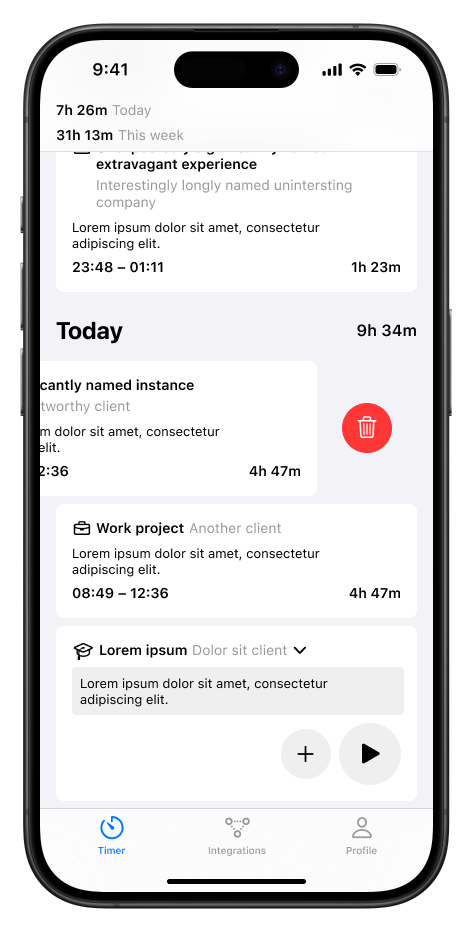
\includegraphics[width=6cm]{timer.png}
		\caption{Časovač}
		\label{fig:timer}
	\end{subfigure}
	\hspace{2cm}
	\begin{subfigure}[b]{0.4\textwidth}
		\centering
		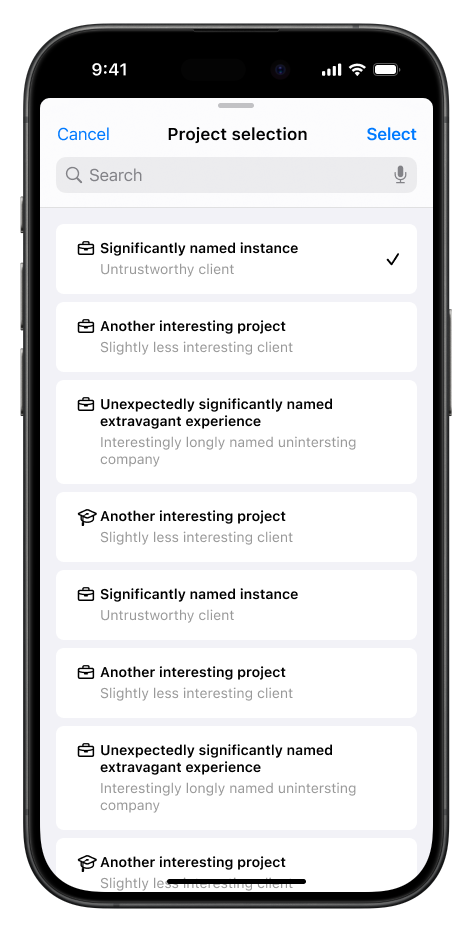
\includegraphics[width=6cm]{project-selection.png}
		\caption{Výběr projektu}
		\label{fig:project-selection}
	\end{subfigure}
	\caption{Hlavní obrazovka}
	\label{fig:timer-and-project-selection}
\end{figure}

Ovládací panel pro časovač může mít různé varianty, jak bude vypadat, podle toho, v~jakém je stavu. Návrh počítá se dvěma možnostmi, jak půjde přidávat časové záznamy do historie:
\begin{itemize}
\item Pomocí časovače – uživatel zapne časovač, když bude chtít začít měření, a poté ho vypne, když bude měření chtít ukončit, čímž se automaticky uloží záznam se zadanými vlastnostmi.
\item Ručně – uživatel ručně zadá začátek a konec záznamu a poté časový záznam uloží.
\end{itemize}
Ovládací panel půjde přepínat mezi těmito dvěma stavy pomocí vedlejšího tlačítka. Hlavní ovládací tlačítko bude vypínat/zapínat časovač, pokud bude přepnut do stavu časovače, nebo bude přidávat ruční záznam, pokud bude v~ručním stavu. V~ovládacím panelu časovače bude také možné vybrat projekt a popis, které budou k~danému záznamu přiděleny. Klik na volbu projektu otevře novou obrazovku, která umožní vyhledávání v~projektech a výběr projektu, jak lze vidět na obrázku \ref{fig:project-selection}. Různé stavy časovače (časovač/manuální, zapnutý/vypnutý, vyplněný/nevyplněný, atd.) lze nahlédnout v~obrázku \ref{fig:timer-control-variants}.

\begin{figure}[h]
	\centering
	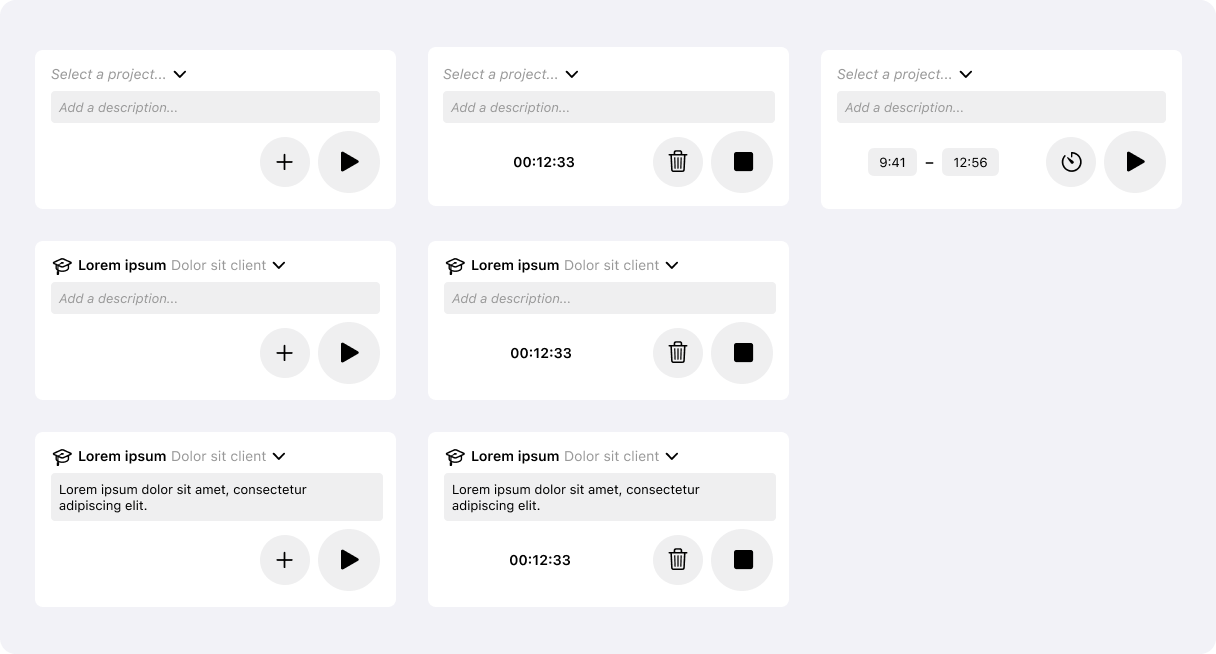
\includegraphics[width=\textwidth]{timer-control-variants.png}
	\caption{Různé stavy ovladače pro časovač}
	\label{fig:timer-control-variants}
\end{figure}

Na obrázku \ref{fig:timer} lze dále v~horní části obrazovky vidět souhrn časových záznam za tento den a týden. Uživatel tak uvidí, kolik času již odpracoval v~daný den i~týden. Časové záznamy v~historii budou také seskupeny podle dnů – každý den bude mít nadpis s~datem a součtem odpracovaného času za ten den. Jednotlivé záznamy také půjdou mazat pomocí posuvného gesta.

Vzhledem k~tomu, že v~historii se může časem nacházet mnoho záznamů, měla by tato obrazovka podporovat stránkování, tedy funkci, že nebude ze zdroje načítat všechny záznamy najednou, ale pouze nějaký kus (stránku), a postupně může načítat další, pokud si to uživatel bude přát. Pokud se během načítání objeví chyba, tak se na této obrazovce ovládací panel časovače ani historie záznamů vůbec nezobrazí – zobrazí se pouze popis chyby a tlačítko pro opakování pokusu o~načtení. Pokud uživatel zatím žádné záznamy mít nebude, tak nebude potřeba zobrazovat nějakou explicitní formu prázdné obrazovky – pouze bude ve spodní části obrazovky ovládací panel a nad tím prázdno.

U~obrazovky pro výběr projektu bude také explicitní chybový stav, který ukáže popis chyby včetně tlačítka pro opakování. Na této obrazovce už ale bude potřeba definovat i~prázdný stav, aby se zobrazila nějaká instrukce, že uživatel nemá vytvořené žádné projekty a musí si je vytvořit na místě k~tomu určeném (bude navrženo dále). Prázdná data lze ale ještě rozdělit do dvou kategorií – prázdná data kvůli tomu, že uživatel žádné projekty nemá, nebo prázdná data kvůli tomu, že jeho vyhledávání neodpovídá žádný projekt. Pro tyto dva stavy je potřeba použít rozdílné texty pro uživatele.

%---------------------------------------------------------------
\subsection{Profil uživatele}\label{feature-profile}
%---------------------------------------------------------------

Profil uživatele bude sloužit pro následující případy užití:
\begin{itemize}
\item\textbf{Zobrazení e-mailové adresy přihlášeného uživatele} – Uživatel si zobrazí e-mailovou adresu účtu, na kterém je přihlášen.
\item\textbf{Odhlášení} – Uživatel se odhlásí ze svého účtu.
\item\textbf{Odstranění účtu} – Uživatel smaže svůj účet.
\item\textbf{Zobrazení projektů} – Uživatel si zobrazí projekty, které má přiřazené.
\item\textbf{Zobrazení klientů} – Uživatel si zobrazí klienty, které má přiřazené.
\item\textbf{Tvorba nebo úprava projektu} – Uživatel si vytvoří projekt nebo upraví existující přiřazený projekt.
\item\textbf{Tvorba nebo úprava klienta} – Uživatel si vytvoří klienta nebo upraví existujícího přiřazeného klienta.
\item\textbf{Odstranění projektu} – Uživatel odstraní projekt, s~ním i~všechny časové záznamy, které pod projekt spadají.
\item\textbf{Odstranění klienta} – Uživatel odstraní klienta, s~ním i~všechny projekty a časové záznamy, které pod klienta spadají.
\end{itemize}

Poslední kartou v~navigační liště aplikace bude karta s~Profilem. Uživatel zde bude mít základní přehled a akce týkající se jeho účtu, jak lze nahlédnout na obrázku \ref{fig:profile-overview}. Uživatel se odsud dostane do seznamu klientů a seznamu profilů, dále si může pomocí tlačítka svůj účet smazat, nebo se odhlásit, což ho vrátí zpět na přihlašovací obrazovku \ref{fig:login}. Mazání účtu je nevratná akce, která vymaže spoustu dat spojených s~uživatelem, je tedy potřeba alespoň ukázat ověřující dialog, který lze nahlédnout na obrázku \ref{fig:profile-delete}. 

\begin{figure}[h]
    \centering
    \begin{subfigure}[b]{0.4\textwidth}
		\centering
		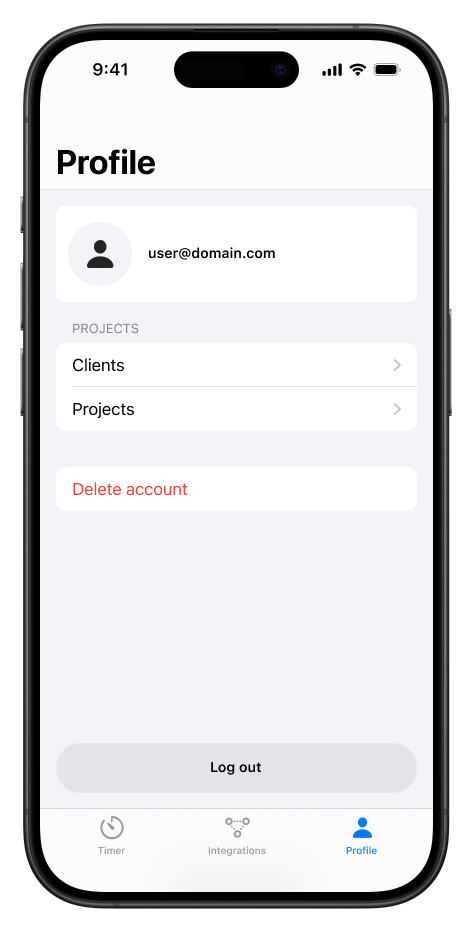
\includegraphics[width=6cm]{profile.png}
		\caption{Přehled}
		\label{fig:profile-overview}
	\end{subfigure}
	\hspace{2cm}
	\begin{subfigure}[b]{0.4\textwidth}
		\centering
		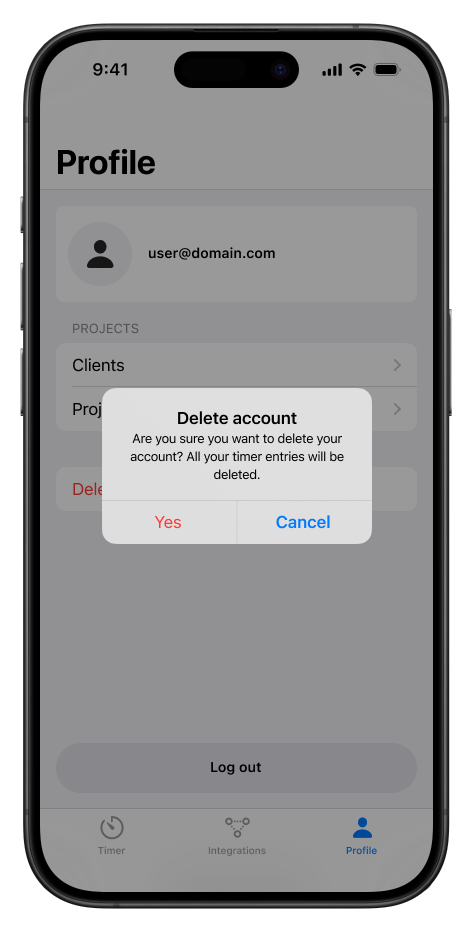
\includegraphics[width=6cm]{profile-delete.png}
		\caption{Smazání účtu}
		\label{fig:profile-delete}
	\end{subfigure}
	\caption{Profil}
	\label{fig:profile}
\end{figure}

V~horní části obrazovky se také nachází uživatelův e-mail, jako indikace toho, na kterém účtě je uživatel přihlášen.

Pokud uživatel klikne na tlačítko klientů, zobrazí se mu seznam jeho klientů, jak lze vidět na obrázku \ref{fig:client-list}. V~tomto seznamu může v~klientech vyhledávat, otevřít detail klienta, nebo vytvořit nového, pomocí tlačítka vpravo nahoře v~navigační liště. Při kliknutí na konkrétního klienta, s~cílem zobrazit jeho detail, i~při kliknutí na volbu tvorby nového klienta, se zobrazí stejná obrazovka detailu, kterou lze nahlédnout na obrázku \ref{fig:new-client}. V~případě zobrazení detailu již existujícího klienta se akorát změní název v~navigační liště, předvyplní se hodnoty klienta a zobrazí se navíc tlačítko pro smazání klienta.

Při tvorbě nebo úpravě klienta uživatel může zvolit jeho název. V~budoucnu je možné přidat další parametry, které by mohly být ke klientovi přiděleny. Kliknutím na tlačítko \emph{Uložit} v~navigační liště se upravený klient uloží a uživatel bude odnavigován zpět na seznam klientů. V~případě, že uživatel klikne na tlačítko zrušit, bude také odnavigován zpět na seznam, ale všechny změny budou zahozeny.

Seznam projektů by měl mít také definované stavy pro chybu a prázdná data. V~případě chyby se zobrazí popis chyby a tlačítko pro opakování, v~případě, že uživatel nemá žádné klienty, se zobrazí tato informace a instrukce k~tomu, aby si nějakého klienta vytvořil. Opět je také potřeba rozlišit mezi tím, zda se žádní klienti nezobrazují proto, protože žádní nejsou, nebo protože žádní nevyhovují vyhledávánému výrazu.

Detail klienta bude mít také explicitní chybový stav, ale prázdný stav zde potřeba není, jelikož existující klient musí mít data vždycky, a nový klient určitě žádná nemá, tudíž budou pole prázdná.

\begin{figure}[h]
    \centering
    \begin{subfigure}[b]{0.4\textwidth}
		\centering
		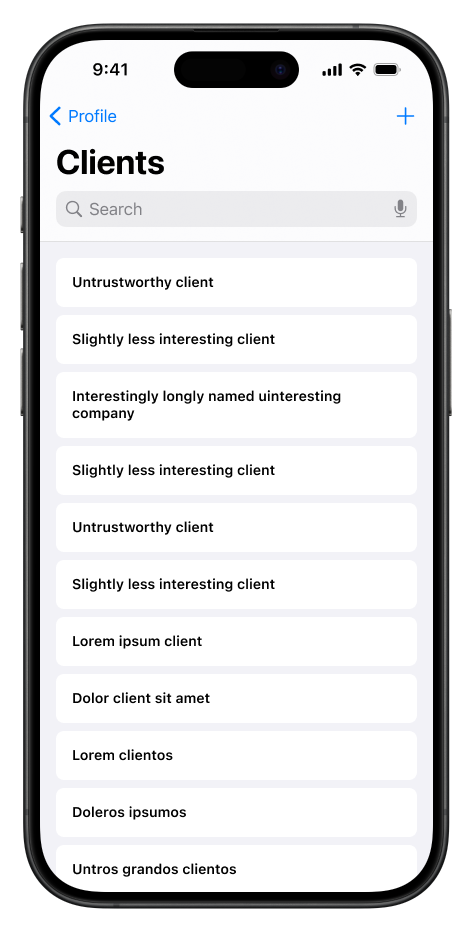
\includegraphics[width=6cm]{clients.png}
		\caption{Seznam}
		\label{fig:client-list}
	\end{subfigure}
	\hspace{2cm}
	\begin{subfigure}[b]{0.4\textwidth}
		\centering
		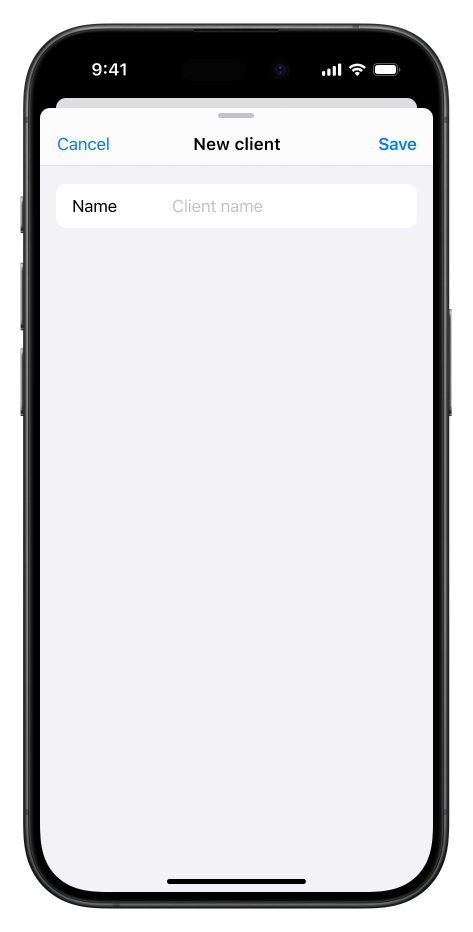
\includegraphics[width=6cm]{new-client.png}
		\caption{Nový klient}
		\label{fig:new-client}
	\end{subfigure}
	\caption{Klienti}
	\label{fig:clients}
\end{figure}

Seznam projektů a detail projektu funguje stejným způsobem, jako u~klientů. Kliknutí na tlačítko projektů v~profilu otevře seznam, odkud lze otevřít detail/tvorbu nového projektu. Seznam projektů lze nahlédnout na obrázku \ref{fig:project-list} a detail projektu na obrázku \ref{fig:new-project}.

Detail projektu narozdíl od klienta obsahuje více informací. Každý projekt musí patřit k~nějakému klientovi, tudíž je potřeba tohoto klienta zvolit, k~čemuž bude sloužit další obrazovka pro výběr klienta, která bude vypadat stejně, jako seznam klientů \ref{fig:client-list}, ale funkčně bude stejná, jako výběr projektu v~časovači \ref{fig:project-selection}. Dále je možnost nastavit jméno projektu, a poté nepovinný údaj o~typu projektu, což bude definovaný seznam hodnot, ze kterého půjde volit (\emph{Práce}, \emph{Škola} a další).

Chybové a prázdné stavy budou fungovat stejným způsobem, jako u~klientů.

\begin{figure}[h]
    \centering
    \begin{subfigure}[b]{0.4\textwidth}
		\centering
		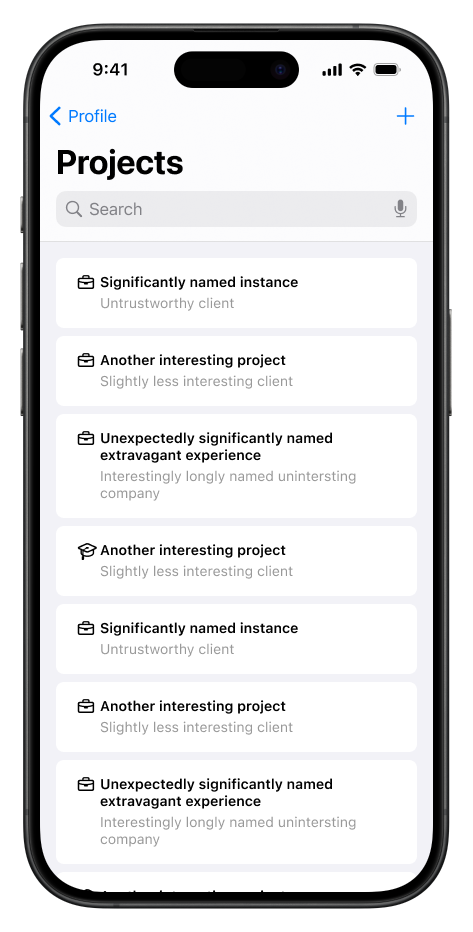
\includegraphics[width=6cm]{projects.png}
		\caption{Seznam}
		\label{fig:project-list}
	\end{subfigure}
	\hspace{2cm}
	\begin{subfigure}[b]{0.4\textwidth}
		\centering
		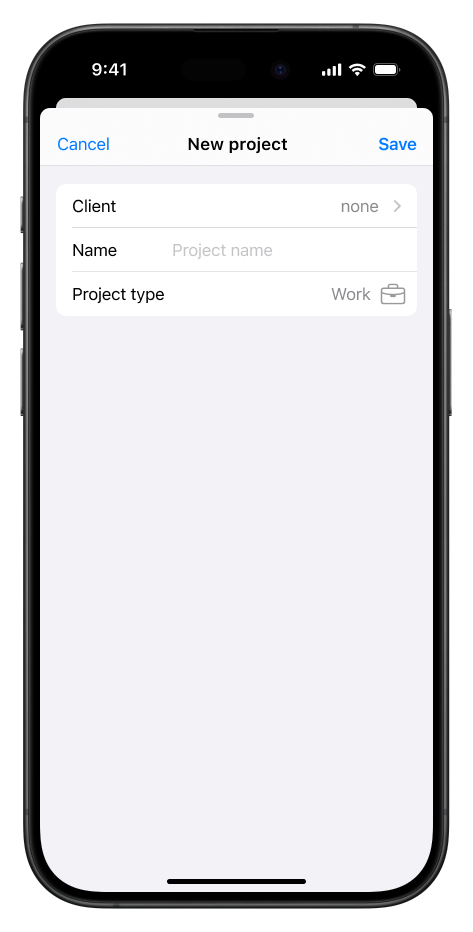
\includegraphics[width=6cm]{new-project.png}
		\caption{Nový projekt}
		\label{fig:new-project}
	\end{subfigure}
	\caption{Projekty}
	\label{fig:projects}
\end{figure}

%---------------------------------------------------------------
\subsection{Integrace}\label{feature-integration}
%---------------------------------------------------------------

Jedním z~cílů práce je stanovit požadavky pro integraci spouštěčů měření času, dále požadavky na integraci aplikace s~existujícími systémy pro měření času, a tyto požadavky v~aplikaci implementovat. Tyto dva typy integrací lze rozdělit do skupin \emph{import} (integrace se spouštěči) a \emph{export} (integrace s~existujícími systémy).

%---------------------------------------------------------------
\subsubsection{Import}\label{feature-integration-import}
%---------------------------------------------------------------

V~sekci \ref{tracking-triggers} byly popsány teoretické možnosti, s~jakými spouštěči by aplikace šla propojit.

Prvním typem spouštěčů měření času byly fyzické spouštěče, tedy nějaké fyzické formy ovladače. Z~uvedených příkladů v~analýze byl pouze jeden, který by uměl uskutečnit napojení na aplikaci napřímo, a to \emph{TIMEFLIP} \cite{timeflip}, který poskytuje protokol pro BLE komunikaci. Implementace BLE komunikace s~hardwarovým produktem je ale poměrně komplexní záležitost, která byla začleněna nad rámec rozsahu této práce, která se už takto věnuje návrhu a implementaci celé platformy pro měření odpracovaného času. Implementace tohoto typu komunikace tedy může být podnětem pro budoucí rozšíření aplikace.

Důležité ale je, aby na takové rozšíření byla aplikace dobře připravená, a aby minimálně poskytovala veřejné API umožňující se z~jakéhokoli budoucího konfigurovatelného hardwarového řešení na aplikaci napojit.

Dalším typem spouštěčů byly softwarové spouštěče, tedy nějaké formy automatizace. V~sekci \ref{software-tracking-triggers} zabývající se tomuto tématu bylo rozebráno několik typů automatizace (podle polohy, času, režimu soustředění, a podobně). Také bylo ale zmíněno systémové řešení pomocí aplikace \emph{Zkratky} \cite{ios-shortcuts-app}, které dokáže automatizaci všech těchto typů vytvořit. \emph{Zkratky} poskytují společné systémové API, které je velmi rozšířené a Apple se snaží vývojáře přesvědčit, aby nějakou část funkcionality aplikace na toto API napojili. Potenciál této platformy je velký, protože její API umožňuje propojování různých procesů navzájem, aplikace si můžou přeposílat výsledky jednotlivých procesů, navazovat na ně a pracovat s~nimi. 

Aplikace se mohou na toto API napojit pomocí definic takzvaných \emph{App Intents}. Apple v~jejich dokumentaci \cite{ios-app-intents} poskytuje podrobné informace k~tomu, jak tyto \emph{App Intents} definovat, jak pro ně vytvářet parametry, a další. Tyto struktury reprezentují nějakou akci aplikace, kterou uživatel může spustit. Nejpoužívanější (podle očekávání) automatizovatelné funkce aplikace budou zapínání časovače, vypínaní časovače a případně rušení časovače. Bylo by tedy vhodné pro tyto tři funkce vytvořit \emph{App Intents}, které uživatelům umožní vytvářet zkratky a automatizace pro jejich spuštění. V~případě zapínání časovače se také naskytuje možnost použití dvou nepovinných parametrů, a to projekt a popis, který bude uživatel chtít k~záznamu přiřadit.

Implementace integrace se systémovými zkratkami umožní rozsáhlou a potenciálně velmi rozšiřovatelnou míru integrace, protože se jedná o~společné systémové API, na které lze napojit jakoukoli aplikaci, a spousta aplikací nějakou formu napojení na zkratky implementuje. U~systémových aplikací to dokonce platí pro všechny – pokrytí automatizovatelných funkcí je zde velmi široké.

Integrace pro import tedy budou sloužit pro následující případy užití:
\begin{itemize}
\item\textbf{Tvorba, úprava nebo odstranění zkratky} – Uživatel si vytvoří, upraví nebo odstraní existující zkratku, která může obsahovat následující akce:
  \begin{itemize}
  \item\textbf{Spuštění časovače} se zadanými parametry.
  \item\textbf{Zastavení časovače} a uložení měřeného záznamu.
  \item\textbf{Zrušení časovače} a zahození měřeného záznamu.
  \end{itemize}
\item\textbf{Tvorba, úprava nebo odstranění automatizace} – Uživatel si vytvoří, upraví nebo odstraní existující automatizaci, která může spouštět vytvořené zkratky.
\item\textbf{Manuální spuštění zkratky} – Uživatel manuálně spustí zkratku, například pomocí hlasového asistenta \emph{Siri}, pomocí \emph{Spotlight} vyhledávání, nebo přímo v~aplikaci \emph{Zkratky}. 
\end{itemize}

%---------------------------------------------------------------
\subsubsection{Export}
%---------------------------------------------------------------

V~sekci \ref{existing-tracking-solutions} byly popsány populární systémy \emph{Clockify}, \emph{Toggl Track} a \emph{Deputy}, které poskytují funkce pro zaznamenávání odpracovaného času. Všechny tyto systémy poskytují možnost importu dat z~CSV souborů, a u~\emph{Clockify} a \emph{Toggl Track} šlo o~velmi podobné formáty.

Možnost exportu z~aplikace do CSV souboru by tedy byla silným nástrojem, pomocí kterého by se záznamy z~aplikace mohly nejen importovat do těchto systémů, ale byla by uživatelům poskytnuta volná možnost, co s~exportovanými daty dělat. V~různých programech by si je mohli dle svého uvážení analyzovat, vizualizovat, a další. Možnost exportu dat do CSV souboru by tedy v~aplikaci neměla chybět. Ideálně by mělo jít o~formát, který půjde importovat jak do systému \emph{Clockify}, tak do systému \emph{Toggl Track}. Systém \emph{Deputy} cílí na trochu jinou cílovou skupinu, napojení na něj by proto nebylo tolik relevantní, jak již bylo popsáno v~sekci \ref{deputy}.

Všechny zmíněné systémy také poskytovaly veřejné API pro napojení na jejich struktury. Zde už se nepůjde spolehnout na nějaké obecné řešení, které bude pasovat na více systémů, ale bude se potřeba na každý systém napojit zvlášť. V~rámci implementace by mohla být vytvořena integrace alespoň s~jedním systémem, a zároveň by implementace mohla být připravena pro rozšíření o~napojení na další systémy.

Integrace pro export tedy budou sloužit pro následující případy užití:
\begin{itemize}
\item\textbf{Zobrazení existujících integrací} – Uživatel si zobrazí vytvořené integrace.
\item\textbf{Tvorba, úprava nebo odstranění integrace} – Uživatel si vytvoří, upraví nebo odstraní integraci.
\item\textbf{Export dat pomocí integrace} – Uživatel pomocí konkrétní integrace exportuje data v~zadaném rozsahu.
\end{itemize}

Rozhraní pro integraci s~dalšími systémy bylo navrženo následovně. V~pořadí druhá, tedy prostřední, karta v~navigační liště bude sloužit pro vytváření integrací. Aby aplikace mohla v~budoucnu podporovat různé typy integrací a zároveň aby si uživatel mohl svá nastavení integrací ukládat, bude hlavní obrazovku integrací představovat seznam již vytvořených integrací, který lze nahlédnout na obrázku \ref{fig:integration-list}.

\begin{figure}[h]
    \centering
    \begin{subfigure}[b]{0.4\textwidth}
		\centering
		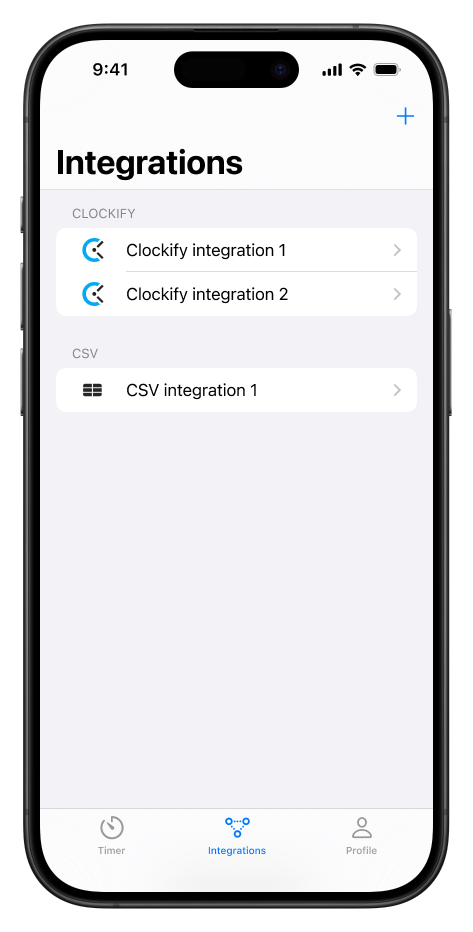
\includegraphics[width=6cm]{integrations.png}
		\caption{Seznam}
		\label{fig:integration-list}
	\end{subfigure}
	\hspace{2cm}
	\begin{subfigure}[b]{0.4\textwidth}
		\centering
		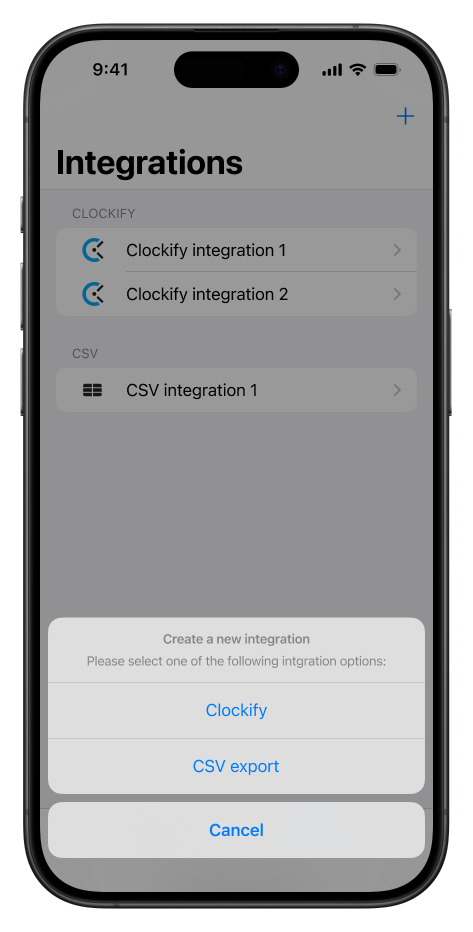
\includegraphics[width=6cm]{new-integration.png}
		\caption{Nová integrace}
		\label{fig:new-integration}
	\end{subfigure}
	\caption{Integrace}
	\label{fig:integrations}
\end{figure}

V~tomto seznamu budou prvky jednotlivých vytvořených integrací, které budou mít přidělenou ikonku podle toho, o~jaký typ integrace se jedná (CSV, \emph{Clockify}, a další). Vpravo nahoře v~navigační liště bude tlačítko pro přidání nové integrace, které otevře dialog s~možnostmi, jaký typ integrace chce uživatel vytvořit, jak lze nahlédnout na obrázku \ref{fig:new-integration}. Tento seznam bude mít definovaný chybový stav, kde se místo seznamu zobrazí popis chyby a tlačítko pro opakování, a prázdný stav, který zobrazí jen informaci o~tom, že si uživatel žádné integrace zatím nevytvořil.

Vytvoření nové integrace, nebo otevření detailu existující integrace, otevře obrazovku pro detail integrace, jak lze vidět na obrázku \ref{fig:clockify-integration}. Obrázek \ref{fig:clockify-integration} reprezentuje detail \emph{Clockify} integrace, u~které je potřeba nastavit název integrace, API klíč pro napojení na \emph{Clockify} účet a případně nějaké další parametry pro exportování dat. Tento detail se bude lišit pro různé typy integrací podle toho, jaké parametry budou pro exportování dat potřeba. Například u~exportu do CSV dat bude potřeba jen název a nic dalšího. Tato obrazovka bude potřebovat definic chybového stavu, který bude opět zobrazovat popis chyby a tlačítko pro opakování. Prázdný stav zde nemá smysl. Obrazovky pro vytvoření nové integrace, nebo pro úpravu existující integrace, se budou lišit akorát v~možnosti odstranění integrace – u~existující integrace se přidá tlačítko, které to umožní.

Kliknutí na tlačítko exportu dat otevře další obrazovku, která lze vidět na obrázku \ref{fig:export-data}. Tato obrazovka bude sloužit pro manuální export dat v~zadaném období. U~některých typů integrací totiž bude dávat smysl nabídnout automatický export dat, například u~\emph{Clockify} integrace, kde je možné každý nově vytvořený záznam rovnou automaticky exportovat do \emph{Clockify} účtu. Ale například u~exportu do CSV souboru taková automatizace nedává smysl, tento typ integrace bude tedy sloužit pouze pro manuální export. Tato obrazovka je poměrně jednoduchá, vyžaduje po uživateli pouze zadání od kdy a do kdy chce časové záznamy exportovat. Pokud zadá validní interval a klikne na tlačítko pro export, aplikace data exportuje. V~případě \emph{Clockify} integrace se pokusí data odeslat na \emph{Clockify} API, v~případě CSV integrace nabídne uživateli výsledný soubor, který si s~ním poté může dělat co chce – uložit do souborů, odeslat e-mailem, otevřít v~jiné aplikaci, atd. U~této obrazovky není potřeba definovat žádné chybové nebo prázdné stavy, protože samotná obrazovka žádná data nepotřebuje.

\begin{figure}[h]
    \centering
    \begin{subfigure}[b]{0.4\textwidth}
		\centering
		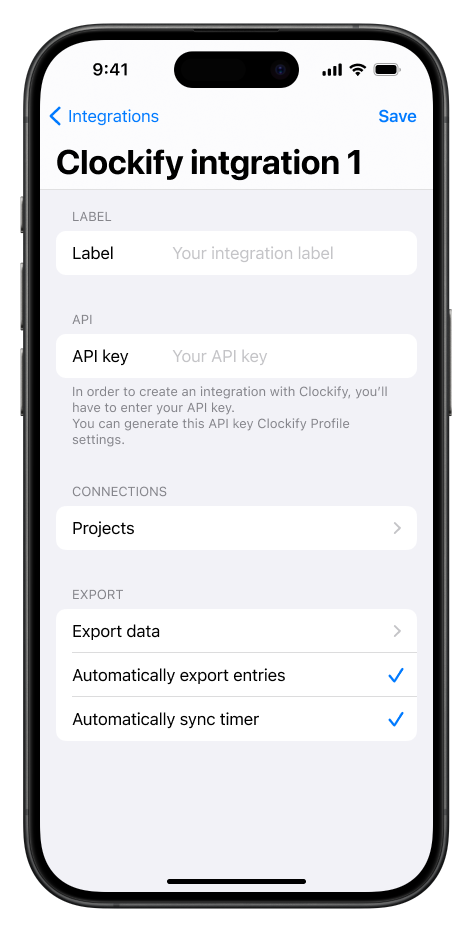
\includegraphics[width=6cm]{clockify-integration.png}
		\caption{Clockify integrace}
		\label{fig:clockify-integration}
	\end{subfigure}
	\hspace{2cm}
	\begin{subfigure}[b]{0.4\textwidth}
		\centering
		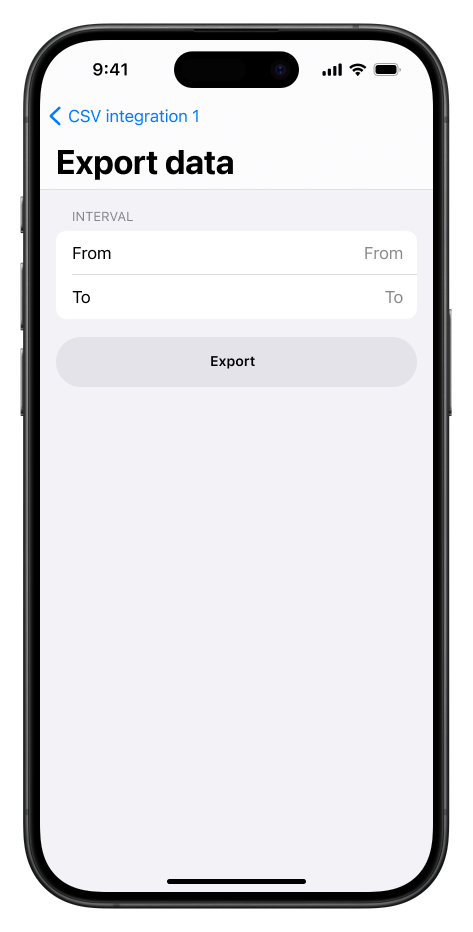
\includegraphics[width=6cm]{export-data.png}
		\caption{Export dat}
		\label{fig:export-data}
	\end{subfigure}
	\caption{Detail integrace}
	\label{fig:integration-detail}
\end{figure}

%---------------------------------------------------------------
\section{Architektura}
%---------------------------------------------------------------

V~analýze v~sekcích \ref{app-architecture}, \ref{crossplatform-multiplatform} a \ref{backend} byly popsány různé architektury pro mobilní aplikace, backendová řešení a databáze. Tato sekce se bude věnovat návrhu architektury celé platformy a nástrojů či jiných produktů, které budou potřeba pro realizaci aplikace.

%---------------------------------------------------------------
\subsection{Architektura platformy}\label{platform-architecture}
%---------------------------------------------------------------

V~první řadě je potřeba se rozhodnout, jakou architekturu bude mít celá platforma, tedy jaký přístup bude zvolen pro vývoj mobilní aplikace, jaké řešení bude zvoleno pro implementaci backendu a jaká bude zvolena implementace databáze. Kombinace těchto řešení lze seřadit na stupnici, která má dva konce:
\begin{itemize}
\item Outsourcování co největší části platformy na externí poskytovale (BaaS, DBaaS, atd.). Tento přístup by byl nejjednodušší z~hlediska komplexní a časové náročnosti implementace, ale ze své podstaty by byl nejvíce omezující ve flexibilitě a možnosti budoucích rozšíření. V~případě, že by bylo v~budoucnu rozhodnuto, že se například změní poskytovatel databáze, tak by bylo značně náročnější implementaci pro takovou změnu upravit. Zejména v~případě, kdyby na jednom externím poskytovateli záviselo více částí infrastruktury.
\item Vlastní implementace všech částí platformy. Toto by vyžadovalo vlastní implementaci nativní aplikace, backendu i~databáze. V~případě, že by bylo v~budoucnu rozhodnuto, že se aplikace rozšíří například o~Android aplikaci, musela by být implementována tato aplikace celá, ale zase by se jen napojila na existující backend. V~tomto ohledu je toto řešení nejvíce flexibilní. Předchozí příklad eventuální změny implementace databáze by byl mnohem jednodušší, pouze by se změnil zdroj dat v~implementaci backendu. Tento přístup by byl ale zásadně náročnější na komplexnost a časovou náročnost implementace. 
\end{itemize}

Vhodné řešení pro implementaci této aplikace bude pravděpodobně ležet někdy mezi těmito dvěma extrémy. Vzhledem k~tomu, že zadání aplikace vyžaduje implementaci aplikace pouze pro platformu iOS, nabízí se lákavé řešení implementovat pouze tuto nativní aplikaci a veškerý zbytek infrastruktury opravdu delegovat na nějaký BaaS. Z~osobních preferencí a kvůli solidní konkurenceschopnosti řešení a jeho obstání jako práce z~dílny oboru softwarového inženýrství se ale toto řešení zdá jako poněkud méně šťastné. Jako jedním z~vedlejších cílů této práce byla zvolena široká možnost budoucích rozšíření této aplikace. Potenciál, kam dále by se implementace dala rozšířit, je široký – aplikace by mohla být rozšířena o~již zmíněnou Android aplikaci, ale třeba také o~webovou aplikaci, nebo o nějakou administrátorskou variantu. Zmíněné řešení s~delegováním celé infrastruktury mimo nativní aplikaci na BaaS by jednoduché řešení těchto rozšíření moc neumožňovala, protože každé další napojení by muselo být implementováno úplně odděleně a muselo by se nějakým způsobem na BaaS napojit, čímž by navíc vznikla silná závislost na poskytovateli BaaS služby.

Zajímavou technologií, která byla zmíněna v~sekci \ref{crossplatform-multiplatform} je \emph{Kotlin Multiplatform} \cite{kotlin-multiplatform}. Z~osobního pohledu tato technologie činí ideální kompromis mezi maximálním využití funkcí jednotlivých platforem a snahy sdílení co největší části kódu. Tato technologie poskytuje nástroje pro sdílení kódu mezi aplikacemi pro různé platformy – iOS, Android, Web a další. Využití této technologie, přestože se realizace bude věnovat pouze implementaci pro platformu iOS, poskytne mnohem jednodušší možnosti pro budoucí rozšíření o~další platformy. Ve sdíleném kódu bude potřeba jen přidat nové moduly podle cílových platforem a bude možnost využít co největší část sdíleného kódu, který je společný pro všechny platformy. Použití této technologie je také osobní preferencí kvůli sympatiím s~jejím používáním, lehkou znalostí práce s~ní a možnost se s~touto technologií více seznámit napřímo.

Rozhodnutí využít technologie \emph{Kotlin Multiplatform} ovlivní i~rozhodnutí při volbě technologie pro implementaci backendu. Pro jazyk \emph{Kotlin} totiž existuje knihovna \emph{Ktor} \cite{ktor}, která poskytuje silné nástroje pro serverovou komunikaci. Poskytuje nástroje jak pro implementaci backendu, tak pro implementaci klienta a jejich vzájemnou komunikaci. Přestože tato knihovna není tak rozšířená a známá jako například \emph{Spring Boot} nebo \emph{Django}, které byly zmíněny v~sekci \ref{backend}, tak se ale hodí pro přehlednost a jednotu zdrojového kódu platformy, kde by celý backend i~multiplatformní část mohla být napsána v~jednom jazyce, v~jednom projektu, v~jednom společném repozitáři.

Rozhodnutí využít nástroje spojené s~multiplatformním vývojem v~\emph{Kotlinu} by se daly využít i~dále. Ve světě vývoje Android aplikací je poslední dobou častou volbou implementace uživatelského rozhraní pomocí knihovny \emph{Jetpack Compose} \cite{compose-ui}. Společnost \emph{JetBrains}, tvůrce technologie \emph{Kotlin Multiplatform}, vyvíjí technologii \emph{Compose Multiplatform} \cite{compose-multiplatform}, která dále umožňuje dokonce implementaci uživatelského rozhraní ve sdíleném kódu, které si narozdíl od cross-platformních řešení stále drží výhody multi-platformního přístupu, tedy lepšího využití možností dané platformy. Tato technologie je ale ve fázi \emph{Alpha} a není tolik pokročilá. Z~toho důvodu zůstala volba pro implementaci uživatelského rozhraní na nativním moderním přístupu s~pomocí knihovny \emph{SwiftUI} \cite{swiftui}.

Zatím tedy padly následující volby – nativní uživatelské rozhraní s~pomocí jazyka \emph{Swift} a knihovny \emph{SwiftUI}, multi-platformní implementace sdíleného kódu s~pomocí technologie \emph{Kotlin Multiplatform}, backend s~pomocí jazyka \emph{Kotlin} a knihovny \emph{Ktor}. Nyní ještě zbývá volba pro implementaci databáze.

V~tomto směru už bylo rozhodnuto, že využití externího DBaaS poskytovatele bude na místě. Toto řešení zjednoduší implementaci aplikace o~technologii vlastní databáze, ale stále si udrží možnost eventuální volby, kdy by se poskytovatel databáze mohl změnit. Jelikož bude mít platforma vlastní backend, nebude problém technologii databáze změnit z~externího poskytovatele například na technologii \emph{PostgreSQL}, protože už to bude jen otázka změny zdroje a migrace dat, zatímco implementace byznysové logiky a dalšího, která bude na backendu, zůstane stejná.

Jako dobrá volba externího poskytovatele BaaS se jeví \emph{Firebase} \cite{firebase} od firmy \emph{Google}. Jedná se o~rozšířenou technologii používanou mnoha aplikacemi. Tato technologie zároveň umožní obsluhu jiných funkcionalit aplikace, jako například autentizace. Není potřeba mezi implementací databáze a autentizace tvořit nějakou závislost, přijde-li tedy v~budoucnu požadavek poskytovatele autentizace nebo databáze změnit, může tak být učiněno nezávisle na sobě, tedy klidně pouze jedno z~toho, nebo obojí.

Tato volba architektury platformy dodržuje požadavek na velkou míru flexibility a rozšiřovatelnosti, zároveň se snaží zjednodušit náročnost implementace a eliminovat duplikace kódu, bude-li aplikace rozšířena o~další platformy. Schéma této architektury lze nahlédnout na obrázku \ref{fig:architecture}. V~tomto obrázku jsou také znázorněny možnosti případného rozšíření aplikace. Z~této celkové architektury platformy lze poté navrhovat architekturu jednotlivých částí.

\begin{figure}[h]
	\centering
	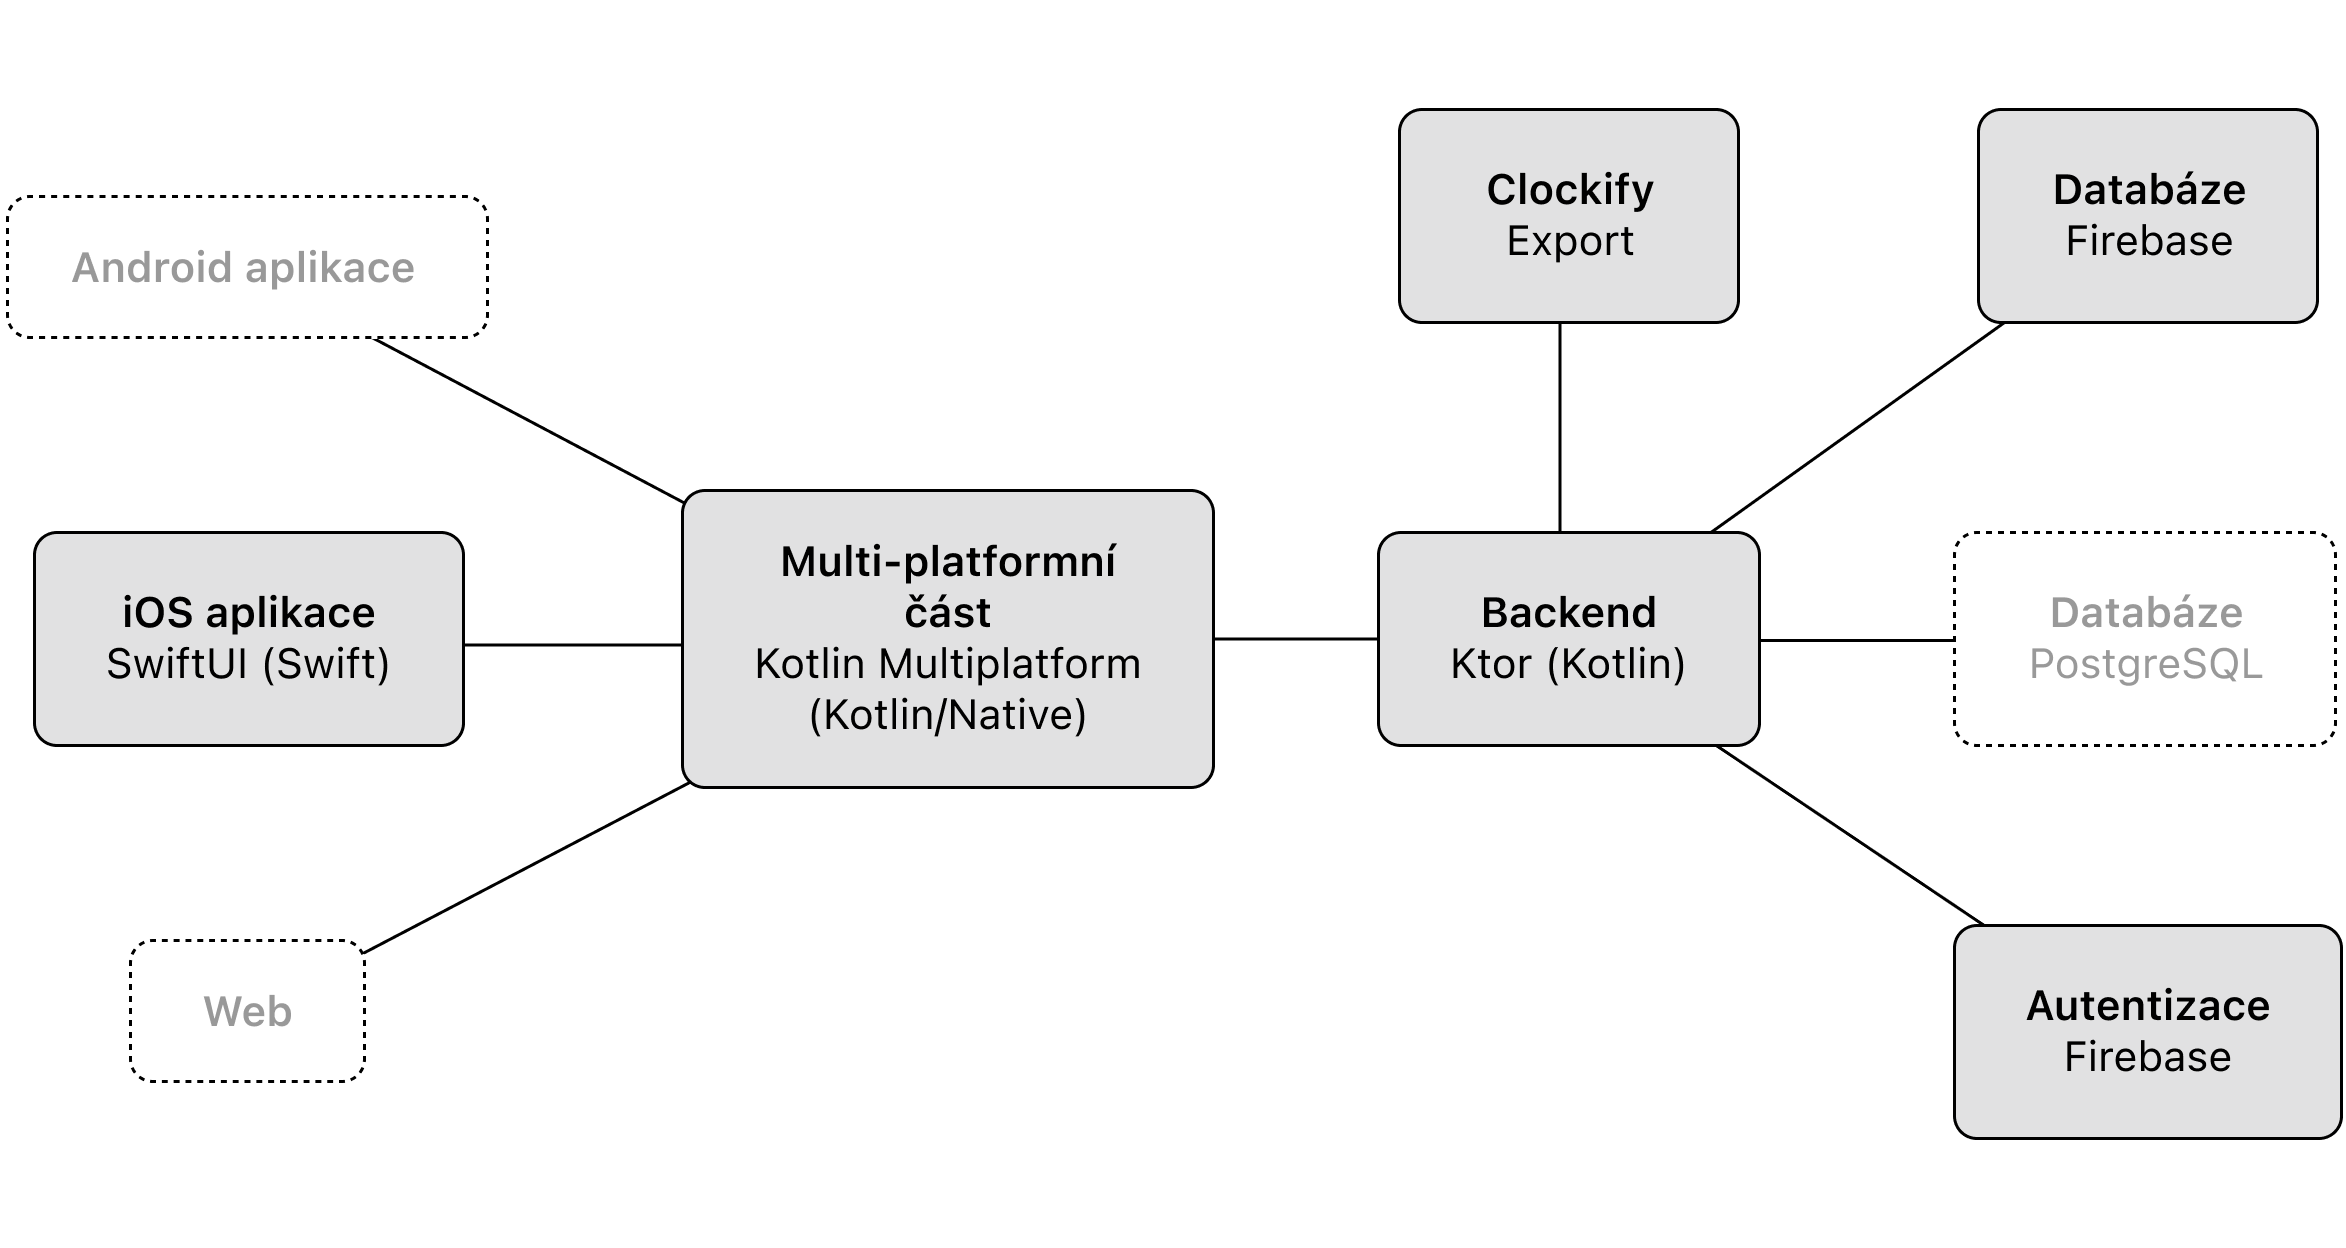
\includegraphics[width=\textwidth]{architecture.png}
	\caption{Architektura platformy}
	\label{fig:architecture}
\end{figure}

%---------------------------------------------------------------
\subsection{Architektura nativní aplikace}
%---------------------------------------------------------------

Architektura nativní aplikace bude vycházet z~veřejné šablony pro projekt mobilní aplikace pro platformy iOS a Android s~použitím technologie \emph{Kotlin Multiplatform}, nazvané \emph{Matee KMP DevStack} \cite{matee-devstack}. Důvody k~použití této platformy jsou osobní preference a znalost tohoto projektu. Alternativou by bylo například použití generátoru šablon projektů \emph{Kotlin Multiplatform Wizard} \cite{kmp-wizard}, ale \emph{DevStack} společnosti \emph{Matee} obsahuje velkou řadu užitečných nástrojů pro uživatelské rozhraní a další užitečné komponenty.

\emph{Matee DevStack} používá architekturu \emph{Clean Architecture} popsanou v~sekci \ref{app-architecture}. Technologie \emph{Kotlin Multiplatform} do této architektury zapadá tak, že nativní aplikace implementuje celou prezentační vrstvu, a multi-platformní část implementuje co největší možnou část doménové a datové vrstvy. Multi-platformní část je do nativní aplikace přidána jako knihovna, která je závislostí doménové vrstvy. Nativní aplikace má tedy přístup hlavně k~doménovým modelům a \emph{Use Cases}.

Nativní aplikace využívá \emph{modularizaci}, která představuje další vlastnost architektury, ve které je aplikace rozdělená do několika modulů, v~tomto případě podle funkcionalit. Prezentační vrstva aplikace tedy bude disponovat moduly podle funkcí jako \emph{Onboarding} (přihlášení/registrace), \emph{Timer} (časovač, historie záznamů), \emph{Integrations} (nastavení integrací), \emph{Profile} (profil uživatele) a poté například modulem \emph{UIToolkit}, který definuje společné komponenty pro prezentační vrstvu.

Doménová vrstva nativní aplikace bude obsahovat moduly \emph{SharedDomain}, což je modul, který definuje společné atributy domény aplikace, ale zde bude mít hlavní funkci jako poskytovatel sdílené knihovny, která bude výstupem multi-platformní části. Dále bude vrstva obsahovat modul \emph{Utilities}, který definuje užitečné nástroje pro práci s~doménovými či sdílenými funkcemi a objekty.

Datová vrstva obvykle obsahuje implementace repozitářů, v~modulech podle funkcionalit, a \emph{Providers}, také v~modulech podle funkcionalit. Jelikož většinu této vrstvy bude implementovat sdílený kód, bude tato vrstva obsahovat jen ty části, které sdílený kód implementovat nemůže. Což jsou obvykle platformní záležitosti, jako obsluha notifikací, GPS polohy, a další. Mohou to být ale i~další implementace, pro které zkrátka multi-platformní část nemá podporu, jako třeba různé funkce poskytovatele \emph{Firebase}. Tyto části kódu budou fungovat tak, že v~multiplatformní části kódu se budou nacházet rozhraní pro funkcionality, které musí implementovat každá platforma sama. V~multiplatformní části se bude pracovat s~těmito rozhraními, a nativní aplikace bude zodpovědná za to, že rozhraním poskytne implementace. Nativní aplikace tedy bude implementovat pouze tu část, kterou sdílená část implementovat nemůže, a výstupy těchto implementací bude vracet do sdíleného kódu.

Zmíněné moduly jsou v~nativní aplikaci ve skutečnosti balíčky typu \emph{Swift Package}, které jsou spravovány nástrojem \emph{Swift Package Manager} \cite{spm}. Nativní aplikace dále obsahuje aplikační vrstvu, která obsahuje základní části aplikace, jako \emph{AppDelegate}, \emph{Info.plist}, ikonu aplikace, nebo například rodičovský \emph{Flow Controller} aplikace, obvykle \emph{AppFlowController}, ze kterého se vytváří všechny další navigační toky. Architekturu nativní aplikace lze nahlédnout na obrázku \ref{fig:app-architecture}.

\begin{figure}[h]
	\centering
	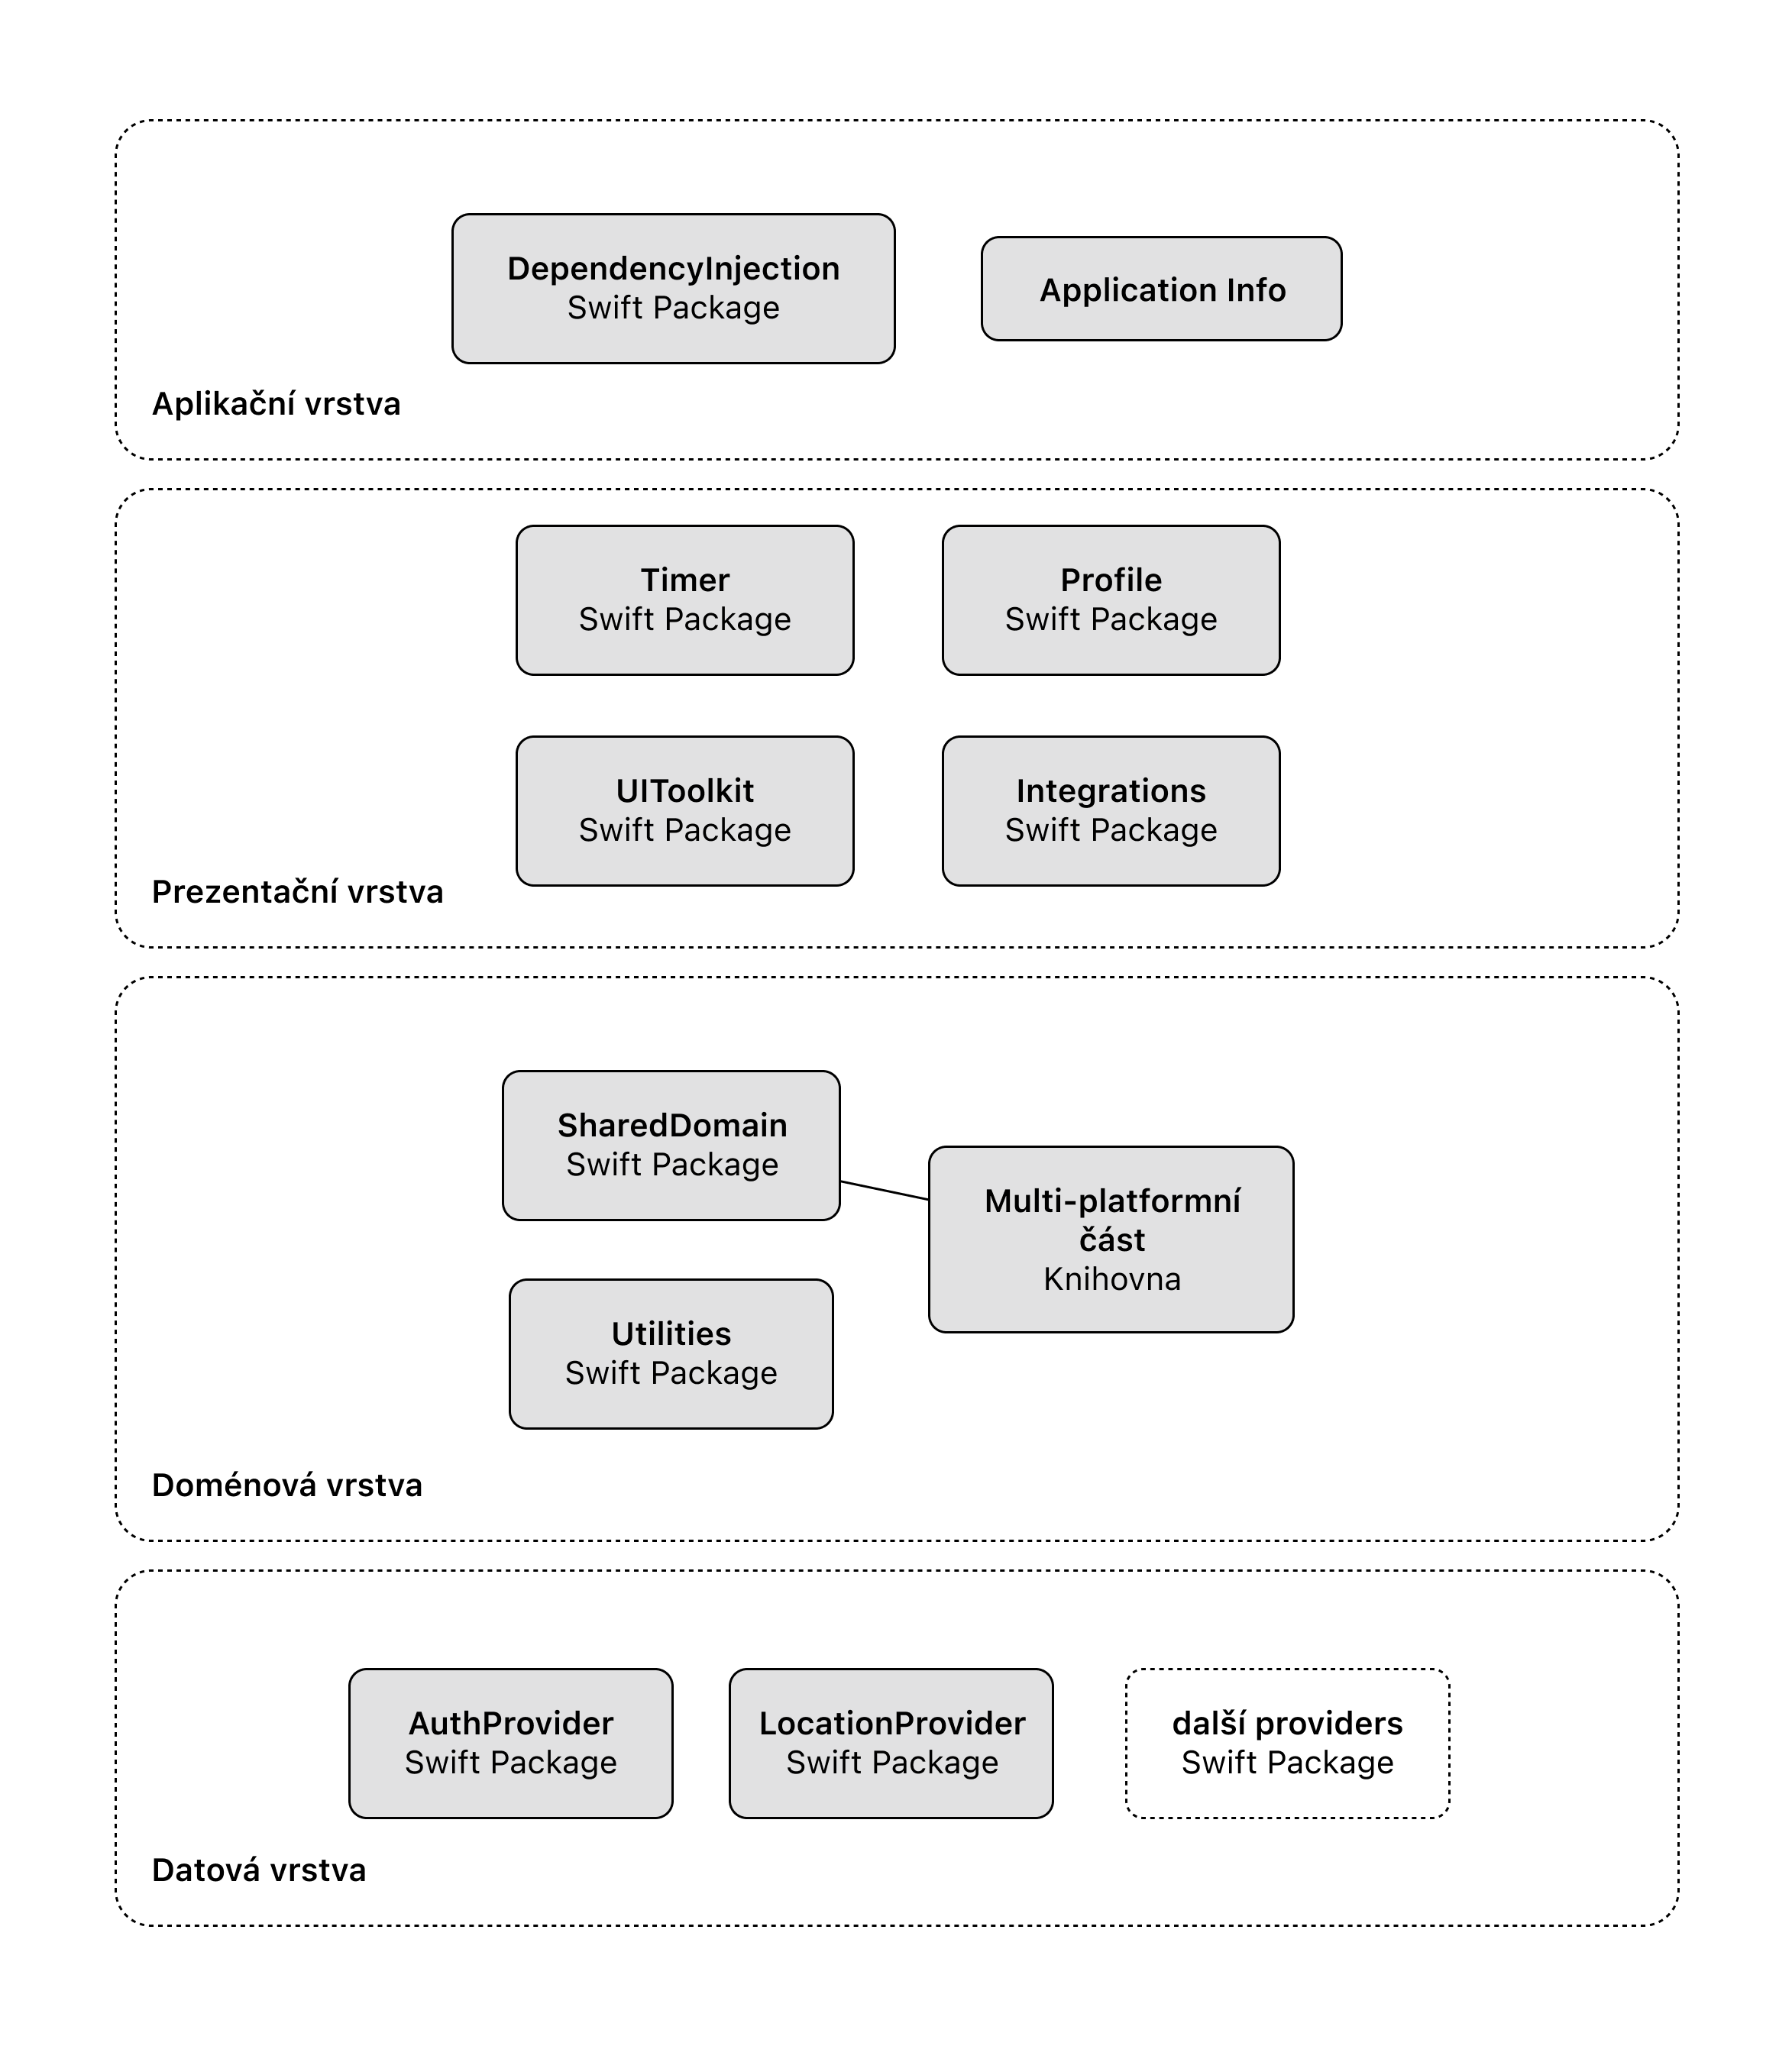
\includegraphics[width=\textwidth]{app-architecture.png}
	\caption{Architektura nativní aplikace}
	\label{fig:app-architecture}
\end{figure}

%---------------------------------------------------------------
\subsection{Architektura multi-platformní části}
%---------------------------------------------------------------

Multi-platformní část je rozdělena do dvou modulů – \emph{commonMain} a \emph{iosMain}. \emph{commonMain} obsahuje sdílený kód všech platforem, a \emph{iosMain} obsahuje kód, který se kompiluje pouze, pokud je cílovou platformou iOS. Toho se využívá speciálními klíčovými slovy v~\emph{Kotlinu} – \texttt{expect} a \texttt{actual}. Funguje to podobně, jako rozhraní – \emph{commonMain} definuje rozhraní funkce/třídy pomocí \texttt{expect}, a platformní modul definuje implementaci pomocí \texttt{actual}. Modul \emph{iosMain} má totiž přístup k~některým platformním API, ke kterým sdílený modul přístup nemá.

Modul \emph{commonMain} poté dodržuje stejnou architekturu, jako nativní aplikace, tedy \emph{Clean Architecture} s~\emph{modularizací} podle funkcionalit aplikace. Jediný rozdíl oproti architektuře používané v~nativní aplikace a popsané v~sekci \ref{app-architecture} je ten, že \emph{Providers} se ve světě \emph{Kotlinu} nazývají \emph{Sources}, ale jejich význam je identický.

Pokud bude v~budoucnu přidána podpora pro další platformy (Android, Web, \dots), bude potřeba v~multi-platformní části přidat konkrétní modul, například \emph{androidMain}. Tyto platformní moduly musí implementovat jen ty části, které jsou specifické pro platformu a \emph{Kotlin/Native} API k~nim má přístup. Dalším specifikem \texttt{expect} a \texttt{actual} je to, že pokud je v~\emph{commonMain} v~nějakém balíčku použito klíčové slovo \emph{expect}, tak v~platformním modulu potom musí být jeho \texttt{actual} implementace ve stejném balíčku. Tedy pokud je například \texttt{expect someFunction(param: String): String} v~balíčku \texttt{com.some.path}, tak implementace potom musí být také v~tomto balíčku. Tím pádem potom musí automaticky platformní moduly reflektovat strukturu aplikace, která je v~\emph{commonMain}.

%---------------------------------------------------------------
\subsection{Architektura backendu}
%---------------------------------------------------------------

Architektura backendu byla zvolena tak, aby byla v~souladu s~\emph{Clean Architecture}, která je používána v~nativní aplikaci i~v~multi-platformní části. Datové a doménové vrstvy jsou tedy identické, s~jednou výjimkou, že v~doménové vrstvě nejsou \emph{Use Cases}, ale ve vyšších vrstvách se budou používat \emph{Repositories} napřímo. To zejména proto, že na backendu mají \emph{Use Cases} menší smysl, než v~aplikaci. Ale nic by nebránilo tomu je také používat. Prezentační vrstva zde bude obsahovat \emph{Routes}, tedy \emph{Endpoints}, se kterými bude moct apikace komunikovat. Jednotlivé \emph{Endpoints} budou přímo volat \emph{Repositories}.

%---------------------------------------------------------------
\subsection{Architektura dat}
%---------------------------------------------------------------

S~ohledem na typ databáze, která byla pro platformu zvolena, je potřeba stanovit nějaké schéma dat. \emph{Firebase} nabízí dva typy databází – \emph{Cloud Firestore} a \emph{Realtime Database}. Oba typy jsou \emph{NoSQL} databáze, \emph{Cloud Firestore} je dokumentová databáze, která ukládá data jako kolekce dokumentů. \emph{Realtime Database} ukládá data v~jednom velkém JSON stromu. Vzhledem k~tomu, že \emph{Cloud Firestore} disponuje oproti \emph{Realtime Database} řadou výhod a je doporučenou variantou, bude tato databáze zvolena pro potřeby aplikace Trackee. \cite{rtdb-vs-firestore}

Jak již bylo řečeno, bude se jednat o~dokumentovou databázi. Pro potřeby aplikace bude nutné definovat následující objekty:
\begin{itemize}
\item\textbf{Klient} – Bude obsahovat informace o~klientovi, v~základní variantě jméno. V~budoucnu může být přidáno více atributů.
\item\textbf{Projekt} – Bude obsahovat informace o~projektu. Projekt musí patřit k~nějakému klientovi, takže bude muset obsahovat identifikátor klienta, ke kterému patří. Dále bude obsahovat jméno a nepovinně typ projektu. V~budoucnu také může být přidáno více atributů.
\item\textbf{Typ projektu} – Předdefinovaný seznam hodnot, například \emph{Práce} nebo \emph{Škola}.
\item\textbf{Uživatel} – Bude obsahovat informace o~uživateli. Identifikátorem uživatele bude \texttt{uid} (User ID), které by mělo být sdíleno s~identifikací v~autentizaci. Dále bude uživatel obsahovat informace o~svém časovači. Poté bude potřeba držet informace o~tom, jaké klienty a projekty má uživatel přiřazené. To by šlo ukládat například pomocí vnořené kolekce, kde bude jednotlivý dokument odpovídat klientovi, a tento dokument bude obsahovat pole hodnot, kterými budou identifikátory projektů, které má od daného klienta přiřazené. A nakonec bude ještě uživatel muset obsahovat data o~svých vytvořených integracích. Ty mohou být uloženy v~další kolekci, kde jednotlivý dokument bude odpovídat integraci.
\item\textbf{Data časovače} – Informace o~tom, jaký má vybraný projekt, popis, zda časovač běží a případně od kdy běží.
\item\textbf{Integrace} – Bude obsahovat název, typ a případně další atributy relevantní k~typu integrace.
\item\textbf{Typ integrace} – Prozatím \emph{CSV} nebo \emph{Clockify}.
\item\textbf{Časový záznam} – Prvek historie časových záznamů, který bude obsahovat informace zadané v~časovači. Tím je tedy vybraný projekt, popis, čas začátku a čas konce.
\end{itemize}
Klient, Projekt, Integrace a Časový záznam budou mít implicitně své identifikátory. U~Uživatele bylo již zmíněno, že jeho identifikátorem bude \texttt{uid}.

Dále je tedy potřeba navrhnout schéma dat. Jelikož se jedná o~dokumentovou databázi, je potřeba ho navrhnout tak, aby nevznikaly zbytečné duplicity a aby byla potřebná data lehce přístupná. Navržené schéma lze nahlédnout na obrázku \ref{fig:data-schema}. 

Schéma je navrženo tak, aby základní objekty byly ukládány ve vlastních top-level kolekcích (\emph{users}, \emph{clients}, \emph{projects} a \emph{entries}). Kolekce \emph{users}, respektive \emph{clients}, obsahují přímo dokumenty jednotlivých uživatelů, respektive klientů, podle jejich identifikátoru. Ale protože \emph{projects} vždy patří k~nějakému klientovi, respektive \emph{entries} k~nějakému uživateli, mají ještě jejich top-level kolekce vnořené kolekce v~dokumentech podle identifikátoru jejich klienta, respektive jejich uživatele. Alternativním přístupem by bylo \emph{projects}, respektive \emph{entries}, ukládat přímo do dokumentů jednotlivých \emph{clients}, respektive \emph{users}, ale tímto způsobem budou dokumenty odlehčeny od obsahování tolika dat a všechny nejpoužívanější objekty domény budou mít své top-level kolekce.

\begin{figure}[h]
	\centering
	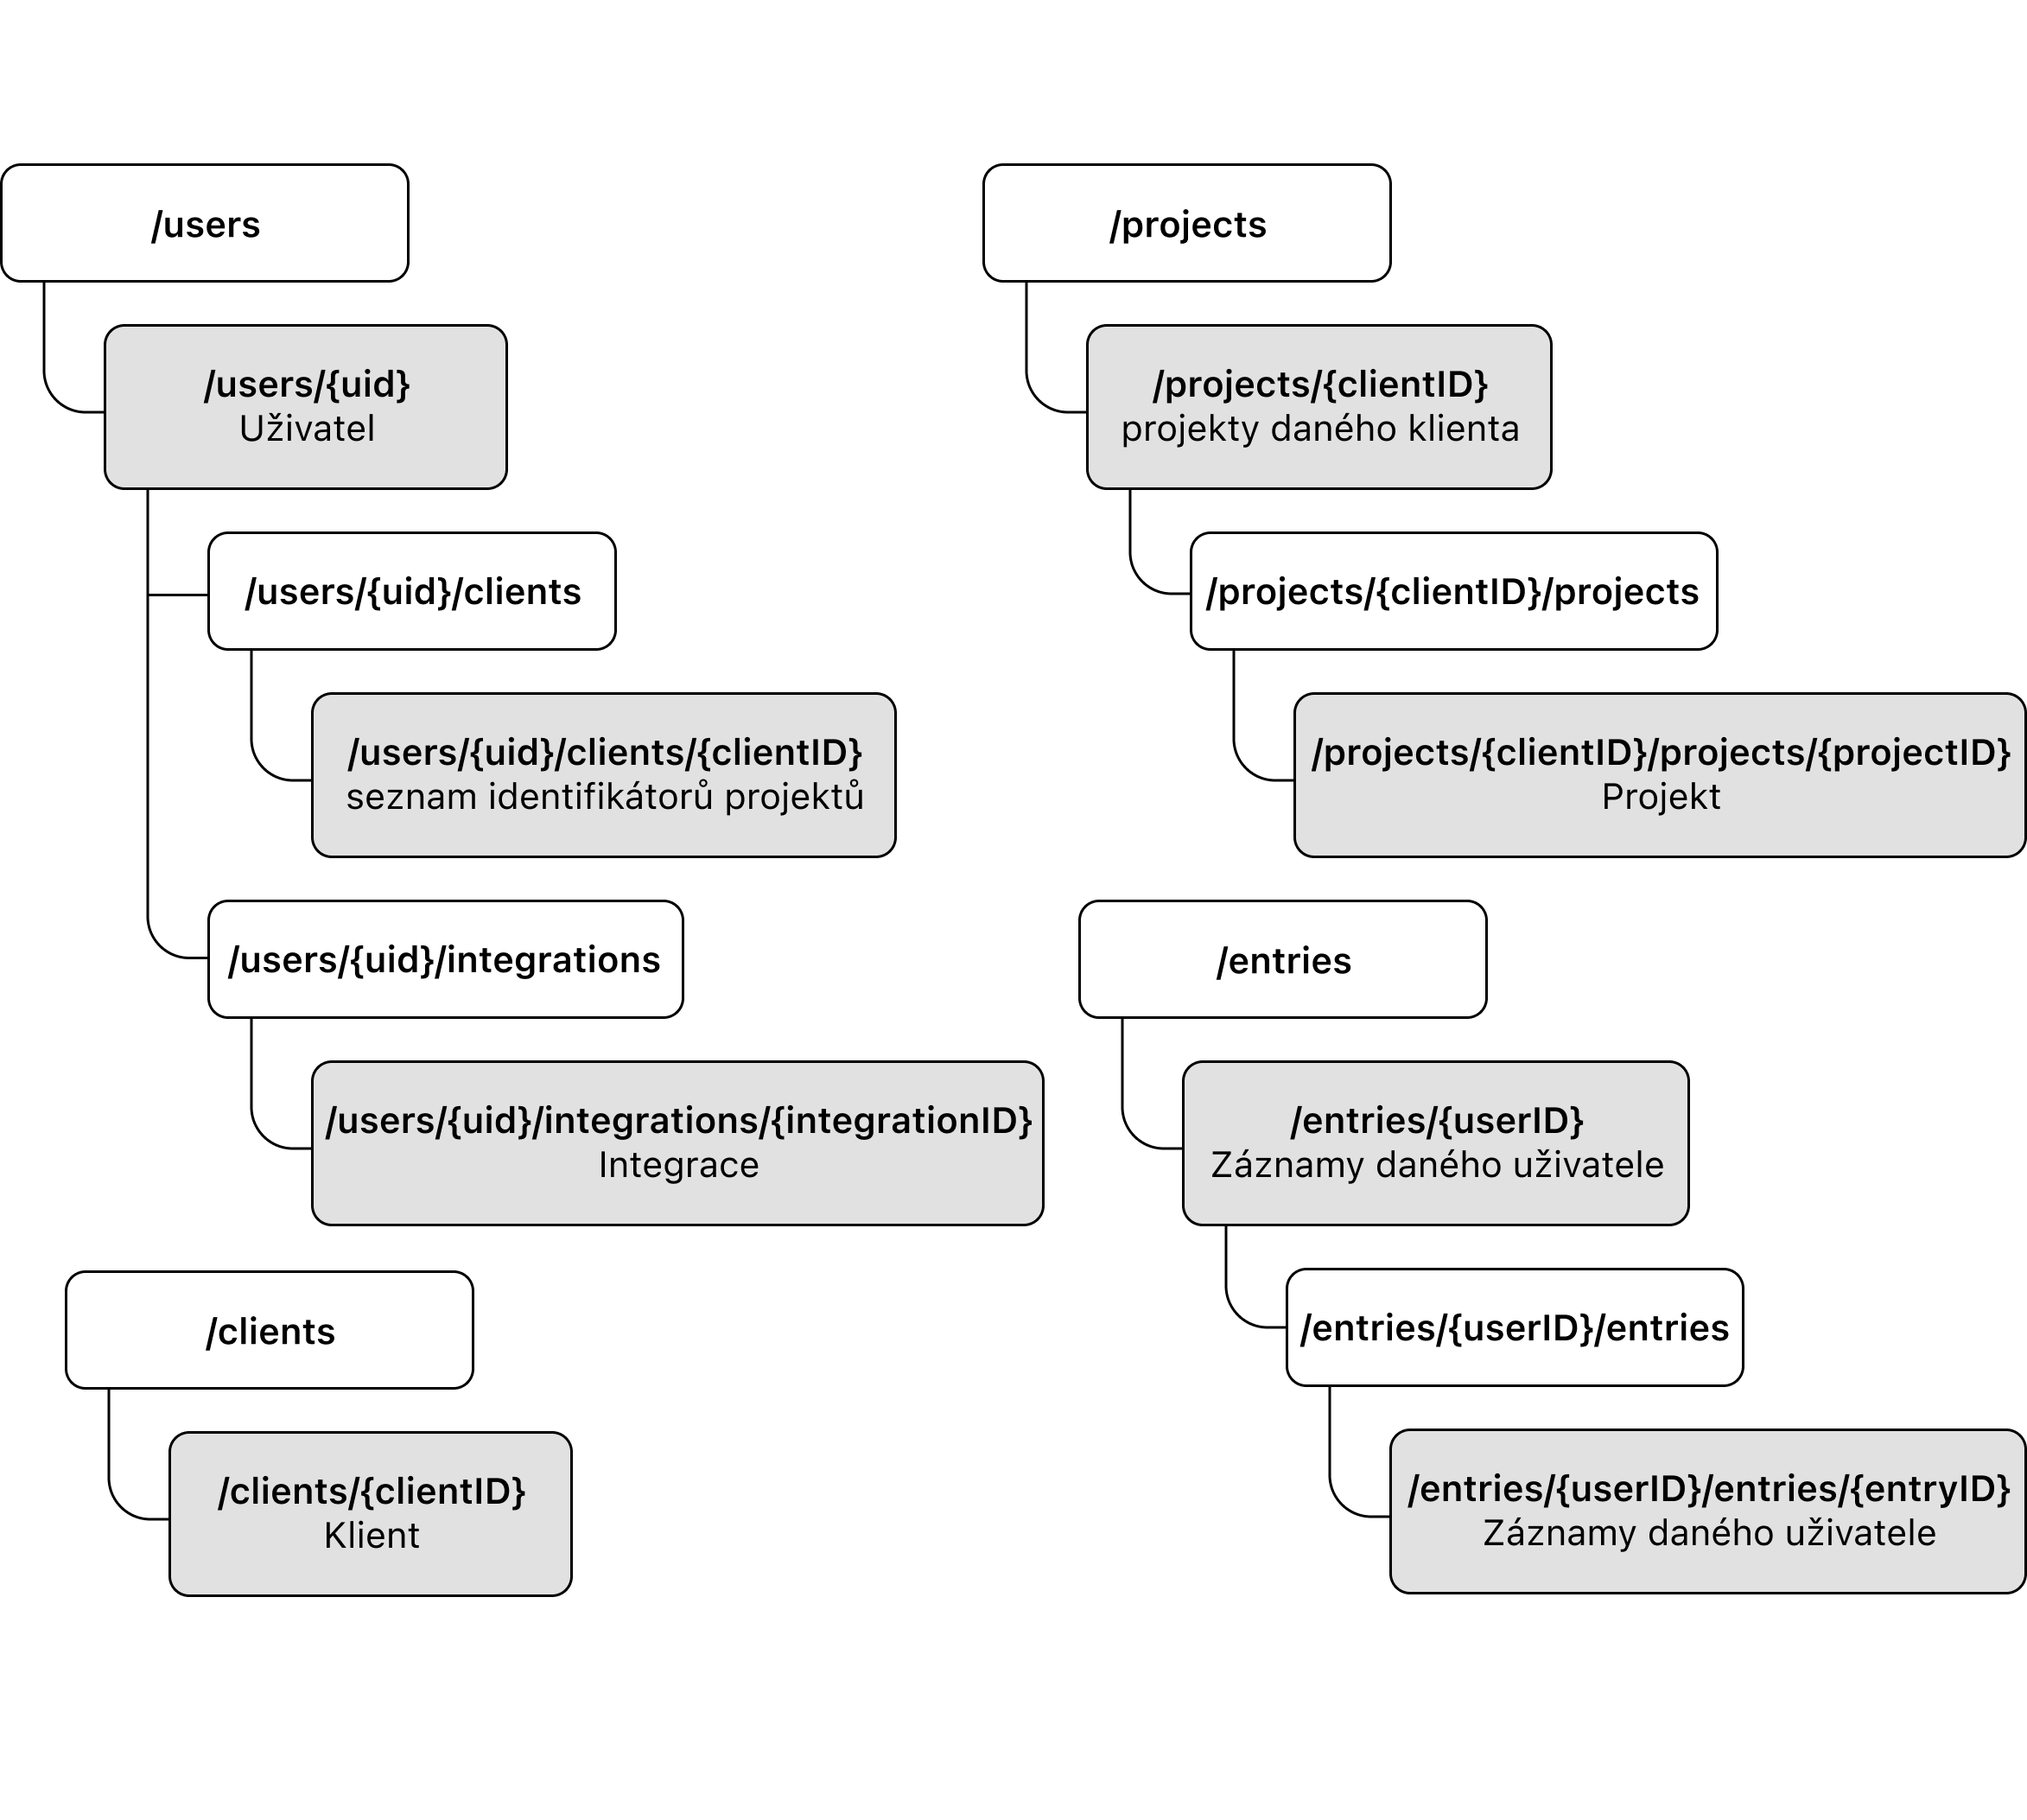
\includegraphics[width=\textwidth]{data-schema.png}
	\caption{Schéma dat}
	\label{fig:data-schema}
\end{figure}

%---------------------------------------------------------------
\section{Nástroje potřebné pro realizaci}\label{dev-tools}
%---------------------------------------------------------------

Před začátkem implementace je také potřeba navrhnout nástroje, které budou pro realizaci potřeba.

U~vývoje nativní aplikace není moc široký výběr vývojových nástrojů, jelikož jediné oficiální vývojové prostředí pro platformu iOS je \emph{Xcode}, popsané v~sekci \ref{ios-dev-tools}, které podporuje pouze operační systém \emph{macOS}. Toto vývojové prostředí obsahuje software pro podporu všech potřebných nástrojů, které jsou pro vývoj pro platformu iOS potřeba – kompilace, archivace, simulátory mobilních zařízení, debugger a další.

Pro vývoj multi-platformní části a backendu bude použito populární vývojové prostředí \emph{IntelliJ IDEA} společnosti \emph{JetBrains} \cite{intellij}. Toto IDE bylo zvoleno z~osobních preferencí a jeho dobré podpoře technologie \emph{Kotlin Multiplatform} i~jazyka \emph{Kotlin}.

Dalším užitečným nástrojem během vývoje bude verzovací systém \emph{Git} \cite{git}, který bude spravovat a verzovat zdrojový kód implementace. 





































